\section{内核功能实现}\label{sec:KernelFunctionalityImplementation}

内核是操作系统的核心组件,负责管理内存和设备,同时为软件应用程序提供使用这些资源的接口。根据复杂性和目标的不同,内核的开发可以遵循不同的模型。主要有两种模型:微内核\footnote{微内核是一种操作系统内核设计,其核心理念是将内核功能最小化,只保留最基本的操作系统服务,如最低级的内存管理、进程调度和通信机制。其他更复杂的服务,如文件系统、网络协议、设备驱动等,则运行在用户空间。}和宏内核\footnote{宏内核则是传统的内核设计方式,将大部分的系统服务和管理功能,如设备驱动、文件系统管理、网络服务等,都直接在内核空间内实现。}。微内核的目标是将大多数服务运行在用户空间,从而提高安全性和模块化。

MinmusOS 采用的是宏内核模式,因此其所有服务和设备驱动程序都在单一地址空间内运行,并处于特权模式下。这种模式提高了效率并减少了代码复杂性,但缺点是其中任何一个组件的错误都可能导致整个系统崩溃。

在本节(\cref{sec:KernelFunctionalityImplementation})中,笔者将详细探讨 MinmusOS 内核各项功能的实现,包括中断管理、驱动程序、多任务处理、系统调用、内存管理、文件系统、计时器以及命令行解释器等。

\subsection{中断(Interrupts)}

中断是操作系统中关键的概念之一,主要用于处理外部设备的信号或内部事件。中断机制使得CPU可以响应并处理紧急事件,同时保持对其他任务的执行。中断主要分为三种类型:

\begin{enumerate}
    \item \textbf{异常(Exceptions)}:同步中断,由CPU执行指令过程中的事件或错误引发,例如除以零错误、执行非法指令或访问无效内存地址。异常通常分为两类:可屏蔽异常和不可屏蔽异常。可屏蔽异常允许操作系统根据当前的需求和优先级来决定是否立即处理。
    \item \textbf{硬件中断(Hardware Interrupts)}:异步中断,由外部硬件设备产生,例如键盘输入、鼠标移动或网络数据包到达。硬件中断使得设备可以通知CPU它们需要立即处理的事件,这对于实时数据处理非常重要。
    \item \textbf{软件中断(Software Interrupts)}:由执行特定的CPU指令集(如INT指令)显式触发,常用于操作系统的系统调用,比如文件访问、网络通信或其他服务请求。软件中断还可以用来执行BIOS(基本输入输出系统)例程,或者其他低级操作。
\end{enumerate}

当中断发生时,CPU会采取以下步骤来处理:

\begin{enumerate}
    \item \textbf{保存当前状态}:CPU首先保存当前正在执行的任务的状态,以便中断处理完成后可以恢复。
    \item \textbf{识别中断类型}:CPU通过查询中断向量表(一个存储了所有中断处理程序入口地址的表格)来识别中断的具体类型和来源。
    \item \textbf{执行中断服务例程(ISR,Interrupt Service Routine)}:每种中断类型都有对应的服务程序。CPU执行这些程序来处理中断。
    \item \textbf{恢复状态}:中断服务完成后,CPU恢复之前中断的任务状态,继续之前的操作。
\end{enumerate}

中断处理机制的设计对于操作系统的效率和响应时间至关重要。优秀的中断处理策略可以显著提高系统的整体性能和用户体验。

\subsubsection{中断描述符表(Interrupt Descriptor Table)}

中断描述符表(IDT)是x86架构中特有的一个关键数据结构,用于管理中断的处理。它的主要目的是提供一个中断服务例程(ISR)的地址映射,当中断发生时,CPU能够知道跳转到哪个位置执行相应的中断处理程序。

IdtEntry 是中断描述符表(IDT)中的基本单元,它定义了每个中断处理函数的具体属性和位置。IdtEntry 结构体的定义如\cref{lst:IdtEntryDataStructure}所示。\texttt{\#[derive(Copy, Clone, Debug)]} 使用 derive 宏为结构体自动实现 Copy、Clone 和 Debug 这三个 trait,\texttt{\#[repr(C, packed)]} 用于指定结构体使用 C 语言风格的内存布局并取消字段对齐,以确保字段在内存中紧凑排列。

\begin{listing}[htbp]
    \begin{minted}{rust}
#[derive(Copy, Clone, Debug)]
#[repr(C, packed)]
pub struct IdtEntry {
    offset_low: u16,       // 偏移地址的低 16 位
    segment_selector: u16, // 中断处理程序代码所在的段选择器
    reserved: u8,          // 保留字段,设置为 0
    flags: u8,             // 位标志
    offset_high: u16,      // 偏移地址的高 16 位
}
    \end{minted}
    \caption{\texttt{IdtEntry}数据结构}\label{lst:IdtEntryDataStructure}
\end{listing}

位标志,包含门类型(Gate Type)、DPL(Descriptor Privilege Level)和 P(Presence):

\begin{enumerate}
    \item \textbf{门类型(Gate Type)}:决定IDT条目是中断门还是陷阱门。例如,0xE(1110b)代表32位中断门。
    \item \textbf{DPL(Descriptor Privilege Level)}:指定可以调用中断的最低特权级(CPL),通常为0,表示只有内核模式可以使用。
    \item \textbf{P(Presence)}:此位必须设置为1,表示此中断向量是有效的。
\end{enumerate}

IdtEntry 结构体提供了 set 方法(\cref{lst:IdtEntrySetMethod})用于设置中断处理程序的地址,这个方法接受一个32位的整数 offset,代表中断处理程序的地址。然后将这个地址分解为两个16位的部分,分别存储到 offset\_low 和 offset\_high。

\begin{listing}[htbp]
    \begin{minted}{rust}
pub fn set(&mut self, offset: u32) {
    self.offset_low = ((offset << 16) >> 16) as u16;
    self.offset_high = (offset >> 16) as u16;
}
    \end{minted}
    \caption{\texttt{IdtEntry}的set方法}\label{lst:IdtEntrySetMethod}
\end{listing}

IdtDescriptor 结构体(\cref{lst:IdtDescriptorDataStructure})定义了一个用于加载中断描述符表(IDT)的描述符。它用于指定 IDT 的大小和内存中的位置,从而允许处理器正确地找到并使用 IDT。size 表示 IDT 的大小,但实际上是 IDT 中最后一个有效条目的偏移量加一。因为中断向量表的条目索引从 0 开始,所以 size 字段的值等于 IDT 的字节长度减一。offset 是一个指向 InterruptDescriptorTable 的指针,表示 IDT 的起始物理地址。这个指针告诉处理器从哪里开始读取中断向量表的数据。

\begin{listing}[htbp]
    \begin{minted}{rust}
#[repr(C, packed)]
pub struct IdtDescriptor {
    size: u16,
    offset: *const InterruptDescriptorTable,
}
    \end{minted}
    \caption{\texttt{IdtDescriptor}数据结构}\label{lst:IdtDescriptorDataStructure}
\end{listing}

InterruptDescriptorTable 结构体(\cref{lst:InterruptDescriptorTableDataStructure})实现了一个关键的系统级数据结构,即中断描述符表(IDT)。这个表是操作系统中管理中断向量的核心结构,用于定义每个中断或异常的处理程序地址。

\begin{listing}[htbp]
    \begin{minted}{rust}
#[repr(C, packed)]
pub struct InterruptDescriptorTable {
    entries: [IdtEntry; IDT_ENTRIES],
}

impl InterruptDescriptorTable {
    pub fn init(&mut self) {
        for i in 0..IDT_ENTRIES {
            self.add(i, exceptions::generic_handler as u32);
        }
    }

    pub fn add(&mut self, int: usize, handler: u32) {
        self.entries[int].set(handler);
    }

    pub fn load(&self) {
        let descriptor = IdtDescriptor {
            size: (IDT_ENTRIES * size_of::<IdtEntry>() - 1) as u16,
            offset: self,
        };
        unsafe {
            asm!("lidt [{0:e}]", in(reg) &descriptor);
        }
    }

    pub fn add_exceptions(&mut self) {
        self.add(0x00, exceptions::division_error as u32);
        ...
        self.add(0x15, exceptions::control_protection_exception as u32);
    }
}
    \end{minted}
    \caption{\texttt{InterruptDescriptorTable}数据结构}\label{lst:InterruptDescriptorTableDataStructure}
\end{listing}

中断描述符表(IDT)的结构体定义与方法实现:

\begin{enumerate}
    \item \textbf{结构体定义}:entries 包含了 IDT\_ENTRIES(256)数量的 IdtEntry 结构体实例。每个 IdtEntry 对应一个中断向量,存储中断处理程序的具体位置和相关属性。
    \item \textbf{init方法}:初始化 IDT 的每个条目,将所有中断向量的处理程序设置为一个通用的处理函数 \texttt{exceptions::generic\_handler}。
    \item \textbf{add方法}:设置特定中断向量的处理程序。它接受中断向量的索引和处理程序的地址(函数指针),然后调用 IdtEntry 的 set 方法来更新相应的条目。
    \item \textbf{load方法}:将 IDT 加载到 CPU 的 IDT 寄存器。它创建一个 IdtDescriptor 结构体,该结构体包含了 IDT 的大小和地址,然后使用 lidt 汇编指令加载这个描述符。
    \item \textbf{add\_exceptions方法}:为常见的 CPU 异常配置特定的处理程序,如除零错误、无效操作码、双重故障、通用保护和页面错误等,中断向量表见\cref{tab:InterruptVectorTable}。
\end{enumerate}

IDT\_ENTRY 是 IdtEntry 类型的静态变量,\cref{lst:IdtEntryTemplate}定义了一个默认的 IDT 条目模板。这个模板被用来初始化 IDT 数组中的每个条目。

\begin{listing}[htbp]
    \begin{minted}{rust}
pub static IDT_ENTRY: IdtEntry = {
    // 段选择器,确定中断处理程序的代码段
    let segment_selector: u16 = {
        let rpl = 0b00 << 0;       // 请求特权级(Ring Privilege Level),0 表示最高权限级别
        let ti = 0b0 << 2;         // 表指示符(Table Indicator),0 表示使用全局描述符表(GDT)
        let index = 0b1 << 3;      // GDT 中的索引,这里是 0x8
        rpl | ti | index           // 组合成完整的段选择器
    };

    // 保留字段,必须设为 0
    let reserved: u8 = 0;

    // 标志位字段,定义了 IDT 条目的属性
    let flags: u8 = {
        let gate_type = 0xe << 0;  // 门类型,0xE 表示 32 位中断门,0xF 表示 32 位陷阱门
        let zero = 0 << 3;         // 保留位,必须为 0
        let dpl = 0 << 5;          // 描述符特权级,0 表示只有内核模式可以使用此中断
        let p = 1 << 7;            // 存在位(Presence bit),1 表示此中断有效
        gate_type | zero | dpl | p // 组合成完整的标志位
    };

    // 构造 IdtEntry 结构体实例
    IdtEntry {
        offset_low: 0,             // 中断处理程序的低 16 位地址,初始化设置为 0,后续指定具体值
        segment_selector,          // 上面定义的段选择器
        reserved,                  // 保留位,始终为 0
        flags,                     // 标志位,定义了 IDT 条目的特性
        offset_high: 0,            // 中断处理程序的高 16 位地址,初始化设置为 0,后续指定具体值
    }
};
    \end{minted}
    \caption{IDT 条目模板}\label{lst:IdtEntryTemplate}
\end{listing}

IDT 是 InterruptDescriptorTable 类型的静态变量,它实际上是一个包含 256 个 IdtEntry 条目的数组。这个数组构成了整个中断描述符表,用于响应各种中断请求。\cref{lst:IDT}使用 IDT\_ENTRY 来初始化每个元素,这意味着每个条目初始时都复制了 IDT\_ENTRY 的设置。特定的中断向量将通过调用 InterruptDescriptorTable 的 add 方法来设置特定的处理函数。

\begin{listing}[htbp]
    \begin{minted}{rust}
pub static mut IDT: InterruptDescriptorTable = InterruptDescriptorTable {
    entries: [IDT_ENTRY; IDT_ENTRIES]
};
    \end{minted}
    \caption{中断描述符表}\label{lst:IDT}
\end{listing}

IDT 定义了操作系统如何响应硬件和软件生成的中断。每个条目对应一个中断向量,系统在收到中断时会查询 IDT 以确定如何处理该中断。通过提供一个统一的方式来处理所有类型的中断,操作系统能够更加有效地管理资源和响应外部事件,从而增强系统的稳定性和响应性。

\subsubsection{中断服务例程(Interrupt Service Routines)}

中断服务例程(ISR)是一种特定的程序,用于处理来自硬件或软件的中断信号。当系统发生中断时,CPU 会自动查找中断描述符表(IDT)中相应的服务例程,并跳转到该例程执行相关操作。与普通的 C 函数不同,ISR 由 CPU 直接调用,并使用特定的 iret 指令返回,这种指令用于恢复中断前的状态,确保系统能安全地继续执行其他任务。

在编写 ISR 时,需要特别注意 CPU 在调用中断服务例程之前会自动将一些寄存器的值压栈,这些寄存器包括 EFLAGS、EIP 和 CS。EFLAGS 寄存器包含了系统的状态标志,EIP 是程序计数器,指示下一条执行指令的地址,CS 是代码段寄存器,指示当前执行代码的段基址。

大部分操作系统使用专门的汇编语言函数来实现中断处理程序,以确保处理过程的高效和准确。MinmusOS 采用 Rust 的内联汇编技术来实现 ISR。这种方法允许在中断服务例程中直接调用其他 Rust 函数,然后通过 iret 指令安全返回,这种技术的使用使得中断处理程序既可以保持高效,也能利用 Rust 语言的安全特性。

\begin{listing}[htbp]
    \begin{minted}{rust}
#[naked]
pub extern "C" fn generic_handler() {
    unsafe {
        asm!(
        "push 0xFF",              // 向堆栈推送一个错误代码
        "call exception_handler", // 调用 exception_handler 函数,用于显示错误信息并处理中断
        "add esp, 4",             // 调整堆栈指针,以清除之前压入的错误代码
        "iretd",                  // 使用中断返回指令,恢复之前由 CPU 自动保存的状态
        options(noreturn),        // 表明汇编代码块执行后不会返回到原始的 Rust 函数中
        );
    }
}
    \end{minted}
    \caption{通用中断处理器}\label{lst:GenericHandler}
\end{listing}

\cref{lst:GenericHandler}定义了一个用于处理多种中断的通用中断服务例程(ISR)。使用 \texttt{\#[naked]} 属性表示这个函数没有由编译器生成的 prologue \footnote{函数的 prologue 是函数实际执行之前的准备阶段。在这个阶段,编译器或者程序会保存旧的基指针、设置新的基指针和为局部变量分配空间。}和 epilogue\footnote{函数的 epilogue 是函数执行完成后的清理阶段。在这个阶段,编译器或者程序会恢复堆栈指针、恢复基指针和返回到调用者。},使得函数可以完全控制所有的堆栈操作。这种处理方式对于中断处理程序来说是必要的,因为它们需要精确控制寄存器和堆栈的状态,但也增加了复杂性和出错的风险。

\begin{listing}[htbp]
    \begin{minted}{rust}
#[no_mangle]
pub extern "C" fn exception_handler(int: u32, eip: u32, cs: u32, eflags: u32) {
    unsafe {
        PRINTER.set_colors(COLOR_WHITE, COLOR_BLUE);
        PRINTER.clear();
    }
    lib::println!();
    lib::println!("  ========== MinmusOS v1.0 ==========                            By Jishen Lin");
    lib::println!();
    lib::println!("  SERIOUS KERNEL ERROR!");
    lib::println!();
    lib::println!("  MinmusOS has encountered a fatal error and the system has been halted.");
    lib::println!();
    lib::println!();
    lib::println!();
    lib::println!();
    lib::println!("  EXCEPTION DESCRIPTION:");
    lib::println!();
    match int {
        0x00 => {
            lib::println!("    DIVISION ERROR!");
        }
        ...
        _ => {
            lib::println!("    EXCEPTION!");
        }
    }
    lib::println!();
    lib::println!();
    lib::println!("  TECHNICAL INFORMATION:");
    lib::println!();
    lib::println!("    ERROR_CODE      : {}", int);
    lib::println!("    INSTRUCTION_PTR : 0x{:X}", eip);
    lib::println!("    CODE_SEGMENT    : 0x{:X}", cs);
    lib::println!("    EXTENDED_FLAGS  : 0b{:b}", eflags);
    lib::println!();
    lib::println!();
    lib::print!("  Please restart your computer. :)");
    loop {}
}
    \end{minted}
    \caption{异常处理器}\label{lst:ExceptionHandler}
\end{listing}

在调试过程中,在代码中通过内联汇编使用 int 命令可以手动触发中断。\cref{lst:ExceptionHandler}为 MinmusOS 提供了友好的用户交互(\cref{fig:ExceptionHandlerPresentation})。蓝屏界面采用了经典的蓝底白字风格,类似于传统的Windows蓝屏死机(BSOD),并显示了详细的错误信息,包括错误类型和技术信息(如错误代码、指令指针、代码段、扩展标志等),有助于开发人员定位问题,便于调试和修复。

\begin{figure}[htbp]
    \centering
    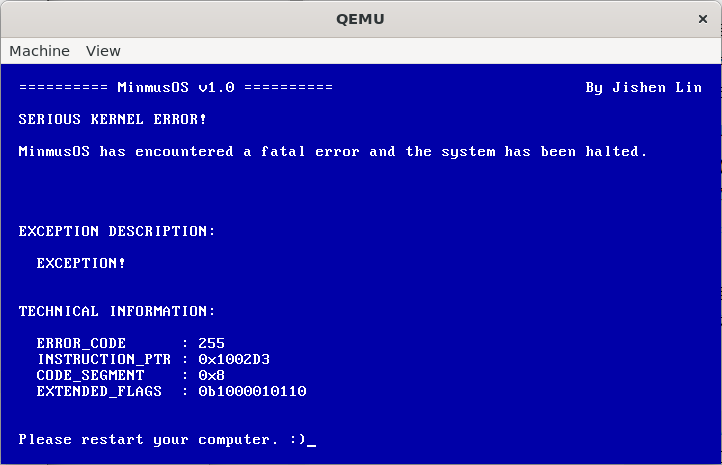
\includegraphics[width=0.8\textwidth]{figures/ExceptionHandlerPresentation.png}
    \caption{异常处理器演示}
    \label{fig:ExceptionHandlerPresentation}
\end{figure}

\subsubsection{CPU 异常(CPU Exceptions)}

异常是 CPU 在执行当前指令过程中遇到错误时自身触发的一种中断。在 x86 架构上,大约有 20 种不同的 CPU 异常类型,见\cref{tab:InterruptVectorTable}。\cref{tab:InterruptVectorTable} 参考自 Intel® 64 和 IA-32 架构软件开发者手册。

\begin{longtable}[c]{@{}llllll@{}}
    \caption{中断向量表}
    \label{tab:InterruptVectorTable}                                                                                                                                                                                                                  \\
    \toprule
    \textbf{向量} & \textbf{助记符} & \textbf{描述}                                                                                                                                            & \textbf{类型} & \textbf{错误代码} & \textbf{来源}                   \\ \midrule
    \endfirsthead
    \multicolumn{6}{r}{\textbf{续表~\thetable}}                                                                                                                                                                                                         \\
    \toprule
    \textbf{向量} & \textbf{助记符} & \textbf{描述}                                                                                                                                            & \textbf{类型} & \textbf{错误代码} & \textbf{来源}                   \\ \midrule
    \endhead
    \hline
    \multicolumn{6}{r}{续下页}
    \endfoot
    \endlastfoot
    0           & \#DE         & 除零错误                                                                                                                                                   & 故障          & 否             & DIV 和 IDIV 指令                 \\
    1           & \#DB         & 调试异常                                                                                                                                                   & 故障/陷阱       & 否             & 指令、数据和 I/O 断点;单步执行等           \\
    2           &              & NMI中断                                                                                                                                                  & 中断          & 否             & 不可屏蔽的外部中断                     \\
    3           & \#BP         & 断点                                                                                                                                                     & 陷阱          & 否             & INT3 指令                       \\
    4           & \#OF         & 溢出                                                                                                                                                     & 陷阱          & 否             & INTO 指令                       \\
    5           & \#BR         & BOUND 范围超出                                                                                                                                             & 故障          & 否             & BOUND 指令                      \\
    6           & \#UD         & 无效操作码(未定义操作码)                                                                                                                                          & 故障          & 否             & UD 指令或保留操作码                   \\
    7           & \#NM         & 设备不可用(无数学协处理器)                                                                                                                                         & 故障          & 否             & 浮点数或 WAIT/FWAIT 指令            \\
    8           & \#DF         & 双重故障                                                                                                                                                   & 中止          & 是(零)          & 任何能生成异常、NMI 或 INTR 的指令        \\
    9           &              & 协处理器段溢出(保留)                                                                                                                                            & 故障          & 否             & 浮点数指令                         \\
    10          & \#TS         & 无效的 TSS\footnote{TSS(Task State Segment)是Intel x86架构中用于任务切换和状态维护的数据结构。它存储了处理器在执行任务时需要的所有状态信息,使得操作系统能够管理多任务环境中的任务切换。TSS的使用主要体现在硬件级别的任务切换和保护模式下的任务状态管理。} & 故障          & 是             & 任务切换或 TSS 访问                  \\
    11          & \#NP         & 段不存在                                                                                                                                                   & 故障          & 是             & 加载段寄存器或访问系统段                  \\
    12          & \#SS         & 栈段故障                                                                                                                                                   & 故障          & 是             & 栈操作和 SS 寄存器加载                 \\
    13          & \#GP         & 通用保护                                                                                                                                                   & 故障          & 是             & 任何内存引用和其他保护检查                 \\
    14          & \#PF         & 页面错误                                                                                                                                                   & 故障          & 是             & 任何内存引用                        \\
    15          &              & (Intel 保留)                                                                                                                                             &             & 否             &                               \\
    16          & \#MF         & x87 FPU 浮点错误(数学故障)                                                                                                                                     & 故障          & 否             & x87 FPU 浮点或 WAIT/FWAIT 指令     \\
    17          & \#AC         & 对齐检查                                                                                                                                                   & 故障          & 是(零)          & 内存中的任何数据引用                    \\
    18          & \#MC         & 机器检查                                                                                                                                                   & 中止          & 否             & 错误代码(如果有)和来源取决于模型             \\
    19          & \#XM         & SIMD 浮点异常                                                                                                                                              & 故障          & 否             & SSE/SSE2/SSE3 浮点指令            \\
    20          & \#VE         & 虚拟化异常                                                                                                                                                  & 故障          & 否             & EPT 违规                        \\
    21          & \#CP         & 控制保护异常                                                                                                                                                 & 故障          & 是             & RET/IRET/RSTORSSP/SETSSBSY 指令 \\
    22-31       &              & (Intel 保留)                                                                                                                                             &             &               &                               \\
    32-255      &              & 用户定义(非保留)中断                                                                                                                                            & 中断          &               & 外部中断或 INT n 指令                \\ \bottomrule
\end{longtable}

\subsubsection{可编程中断控制器(Programmable Interrupt Controller)}

可编程中断控制器(Programmable Interrupt Controller,简称 PIC),尤指 8259 PIC,是早期计算机主板上用于管理硬件中断的一个小型芯片。在现代计算机中,这一芯片通常已被整合进 CPU 的设计中。PIC 的核心作用是接收来自硬件设备的中断信号,并在 CPU 准备接收时,将这些信号有效地分派给 CPU,从而响应外部设备的事件或请求。

PIC 有 28 个引脚,其中 8 个引脚是中断输入线,用于连接那些可以触发中断的硬件组件。这些中断线路将外部设备如键盘、鼠标或其他I/O设备的中断请求直接传输到 PIC。由于单个 PIC 只能处理有限的 8 个中断,现代计算机系统为了扩展中断处理能力,通常会使用两个 PIC 芯片,配置为一主一从模式。这种配置允许系统处理更多的中断线路,总共可达 15 个中断(一个用于连接主从 PIC)。虽然现代计算机系统普遍采用了更为先进的高级可编程中断控制器(APIC),以支持更大数量的中断线路和更复杂的中断管理功能,PIC 依旧因其向后兼容性而被支持在新的系统中,确保老旧硬件和软件的正常运行。

CPU 在设计时已经为处理器内部的异常(如除零错误、访问违规等)预留了前 32 个中断向量。因此,来自外部硬件的中断必须被映射到 32 号以上的中断向量,以避免与这些处理器异常冲突。

重新映射中断是通过向 PIC 的命令和数据端口发送特定的命令来完成的。对于主 PIC,其命令端口位于 0x20,数据端口位于 0x21;从 PIC 的命令端口位于 0xA0,数据端口位于 0xA1。初始化 PIC 时,会发送一个初始化命令,设定中断向量的偏移量,指定哪个是主 PIC,哪个是从 PIC,并设置运行模式。

可编程中断控制器(Programmable Interrupt Controller)驱动程序的实现见\cref{sec:ProgrammableInterruptControllerDriver}。

\subsection{驱动程序(Drivers)}

设备驱动程序是一种软件组件,其目的是使特定的硬件设备与内核进行接口交互。默认情况下,操作系统并不知道如何与硬件通信,因此需要驱动程序将操作系统的请求转换成硬件能够理解和执行的命令。

\subsubsection{可编程中断控制器驱动程序(Programmable Interrupt Controller Driver)}\label{sec:ProgrammableInterruptControllerDriver}

kernel/src/drivers/pic.rs 定义了一个用于管理可编程中断控制器(Programmable Interrupt Controller,PIC)的驱动程序,特别针对老式的 8259 PIC 设计。这些 PICs 主要用于中断管理,使得硬件中断能被适当地映射并处理。

相关常量定义如下:

\begin{enumerate}
    \item \texttt{MASTER\_PIC\_COMMAND\_PORT}:主 PIC 接收命令的端口地址是 0x20
    \item \texttt{MASTER\_PIC\_DATA\_PORT}:主 PIC 数据读写的端口地址是 0x21
    \item \texttt{SLAVE\_PIC\_COMMAND\_PORT}:从 PIC 接收命令的端口地址是 0xA0
    \item \texttt{SLAVE\_PIC\_DATA\_PORT}:从 PIC 数据读写的端口地址是 0xA1
    \item \texttt{COMMAND\_INIT}:用于初始化 PIC 的命令字节,其值为 0x11
    \item \texttt{COMMAND\_EOF}:用于告诉 PIC 中断处理完成的命令字节,其值为 0x20
    \item \texttt{MODE}:设置 PIC 的工作模式为 8086 模式,其值为 0x01
    \item \texttt{OFFSET}:定义中断向量表中断向量的起始偏移量,这里设为 32,这是因为 0-31 号中断已被 CPU 的异常占用
    \item \texttt{IRQ\_COUNT}:每个 PIC 能够处理的中断数量,这里设为 8,表示每个 PIC 可以管理 8 个中断
\end{enumerate}

\cref{lst:MasterSlavePICInstance}定义了一个名为 PICS 的静态变量,它是 Pics 类型的实例,代表系统中的主从可编程中断控制器(PIC)。该实例包括两个 Pic 结构体,分别配置了主和从 PIC 的中断偏移量、命令端口和数据端口。此静态变量在整个程序运行期间全局可访问,用于初始化和管理硬件中断,确保操作系统能够正确响应外部设备的中断请求。

\begin{listing}[htbp]
    \begin{minted}{rust}
pub static PICS: Pics = Pics {
    master: Pic {
        offset: OFFSET,
        command_port: MASTER_PIC_COMMAND_PORT,
        data_port: MASTER_PIC_DATA_PORT,
    },
    slave: Pic {
        offset: OFFSET + IRQ_COUNT,
        command_port: SLAVE_PIC_COMMAND_PORT,
        data_port: SLAVE_PIC_DATA_PORT,
    },
};
    \end{minted}
    \caption{主从可编程中断控制器(PIC)实例}\label{lst:MasterSlavePICInstance}
\end{listing}

\cref{lst:PicDataStructure}定义了一个可编程中断控制器(PIC)的基本属性和操作方法。这个结构体和其方法主要用于对硬件中断进行低级控制,允许操作系统正确地响应外部中断请求。

\begin{listing}[htbp]
    \begin{minted}{rust}
struct Pic {
    offset: u8,       // 中断向量的起始偏移量,这个偏移量是中断向量表中该 PIC 控制的中断开始位置
    command_port: u8, // PIC 的命令端口地址
    data_port: u8,    // PIC 的数据端口地址
}

impl Pic {
    // 从 PIC 的数据端口读取一个字节的数据
    pub fn read_data(&self) -> u8 {
        let data: u8;
        unsafe {
            asm!("in al, dx", out("al") data, in("dx") self.data_port as u16);
        }
        data
    }

    // 将数据写入到 PIC 的数据端口
    pub fn write_data(&self, data: u8) {
        unsafe {
            asm!("out dx, al", in("dx") self.data_port as u16, in("al") data);
        }
    }

    // 向 PIC 的命令端口发送指定的命令
    pub fn send_command(&self, command: u8) {
        unsafe {
            asm!("out dx, al", in("dx") self.command_port as u16, in("al") command);
        }
    }

    // 通知 PIC 一个中断处理已经结束
    pub fn end_interrupt(&self) {
        unsafe {
            asm!("out dx, al", in("dx") self.command_port as u16, in("al") COMMAND_EOF);
        }
    }

    // 检查给定的中断号是否由当前的 PIC 处理,判断依据是中断号是否位于该 PIC 的控制范围内
    pub fn handles_interrupt(&self, interrupt: u8) -> bool {
        self.offset <= interrupt && interrupt < self.offset + IRQ_COUNT
    }
}
    \end{minted}
    \caption{\texttt{Pic}数据结构}\label{lst:PicDataStructure}
\end{listing}

\cref{lst:PicsDataStructure}定义了一个包含两个可编程中断控制器(PIC),即主 PIC 和从 PIC 的组合。该结构体及其方法的设计与实现主要用于系统中断管理,允许系统初始化和管理来自硬件的中断信号。

\begin{listing}[htbp]
    \begin{minted}{rust}
pub struct Pics {
    master: Pic, // 主 PIC
    slave: Pic,  // 从 PIC
}

impl Pics {
    // 初始化
    pub fn init(&self) {
        // 读取当前的中断屏蔽状态
        let mask1 = self.master.read_data();
        let mask2 = self.slave.read_data();
        // 向每个 PIC 发送初始化命令
        self.master.send_command(COMMAND_INIT);
        wait();
        self.slave.send_command(COMMAND_INIT);
        wait();
        // 设置偏移量
        self.master.write_data(self.master.offset);
        wait();
        self.slave.write_data(self.slave.offset);
        wait();
        // 向主 PIC 发送一个数值 4,表示从 PIC 通过主 PIC 的 IRQ2 连接,配置主 PIC 知道如何与从 PIC 通信
        self.master.write_data(4);
        wait();
        // 向从 PIC 发送一个数值 2,指定它是通过主 PIC 的 IRQ2 接入的,为从 PIC 配置连接到主 PIC 的方式
        self.slave.write_data(2);
        wait();
        // 配置为 8086 模式
        self.master.write_data(MODE);
        wait();
        self.slave.write_data(MODE);
        wait();
        // 最终恢复初始屏蔽状态
        self.master.write_data(mask1);
        self.slave.write_data(mask2);
    }

    // 检查指定的中断号是否由当前 Pics 实例的主或从 PIC 处理。此方法为中断服务例程提供决策支持,决定是否需要响应某个特定中断
    pub fn handles_interrupt(&self, interrupt: u8) -> bool {
        self.master.handles_interrupt(interrupt) || self.slave.handles_interrupt(interrupt)
    }

    // 通知 PIC 中断处理已经结束。如果从 PIC 处理了中断,则先通知从 PIC,然后无论如何都通知主 PIC
    pub fn end_interrupt(&self, interrupt: u8) {
        if self.handles_interrupt(interrupt) {
            if self.slave.handles_interrupt(interrupt) {
                self.slave.end_interrupt();
            }
            self.master.end_interrupt();
        }
    }
}
    \end{minted}
    \caption{\texttt{Pics}数据结构}\label{lst:PicsDataStructure}
\end{listing}

在与硬件通信时,尤其是在初始化或配置硬件如可编程中断控制器(PIC)时,必须确保在发送连续的配置命令之间有足够的时间间隔,让硬件有机会响应每个命令。wait 函数(\cref{{lst:PicWaitFunction}})通过向一个通常未使用的端口(0x80)写入一个值(通常是0),来创造一个小的延时,这样的操作需要硬件访问时间,从而实现延迟的目的。

\begin{listing}[htbp]
    \begin{minted}{rust}
pub fn wait() {
    unsafe {
        asm!("out dx, al", in("dx") 0x80u16, in("al") 0u8);
    }
}
    \end{minted}
    \caption{wait函数}\label{lst:PicWaitFunction}
\end{listing}

设计与实现考量:

\begin{enumerate}
    \item \textbf{安全与底层访问}:由于直接与硬件端口交互,多数操作都在 unsafe 块中执行,这符合 Rust 的安全原则,仅在必要时放宽规则。
    \item \textbf{中断管理}:Pics 结构体及其方法设计考虑了中断的优先级和处理流程,确保系统对中断的响应既快速又正确。
    \item \textbf{灵活性和扩展性}:通过独立控制每个 PIC,系统可以灵活地配置中断处理,适应不同的硬件和系统需求。
\end{enumerate}

\subsubsection{键盘驱动程序(Keyboard Driver)}

键盘驱动程序是计算机操作系统中的一个重要组件,负责处理和解释来自物理键盘的输入信号。无论是传统的PS/2键盘还是现代的USB键盘,驱动程序都扮演着至关重要的角色。以下是键盘驱动程序的几个主要功能和特点:

\begin{enumerate}
    \item \textbf{信号解析}:键盘驱动程序首先需要从键盘控制器读取扫描码,这些扫描码是键盘在按键操作时生成的。这些扫描码包含关于哪个键被按下或释放的信息。
    \item \textbf{中断处理}:当按键操作发生时,键盘会向计算机发送一个中断信号,这个信号会触发操作系统中断处理程序。键盘驱动程序必须能够响应这些中断,并从键盘控制器中读取相应的扫描码。
    \item \textbf{数据转换}:驱动程序读取到扫描码后,需要将其解析并转换成具体的键盘事件,如按键按下或释放。这个过程涉及到将扫描码映射到特定的键盘布局和语言设置。
    \item \textbf{事件传递}:解析完成后,驱动程序会生成一个或多个高级的输入事件,这些事件将被操作系统接收并传递给相应的应用程序处理。
    \item \textbf{兼容性和模拟}:对于使用PS/2接口的旧键盘,现代主板通常通过模拟方式支持,将这些设备表现为PS/2设备,以便支持旧软件。这种模拟也需要键盘驱动程序处理特定的兼容性问题。
\end{enumerate}

MinmusOS的PS/2键盘驱动程序负责处理来自PS/2键盘的输入,将扫描码(scancode)转换为ASCII字符,并相应地更新系统状态。该驱动程序利用中断请求(IRQ1,即键盘中断)来响应键盘事件,确保即使在多任务环境下也能及时处理键盘输入。

Keyboard结构体是键盘状态的主要表示形式,包含了各种键盘修饰键的状态(如Shift、Ctrl、Alt和Caps Lock)。这些状态用布尔值表示,分别对应左右Shift键、左右Ctrl键、左右Alt键及Caps Lock键的开关状态。该结构体通过\cref{lst:KeyboardDataStructure}定义。

\begin{listing}[htbp]
    \begin{minted}{rust}
pub struct Keyboard {
    left_shift: bool,
    right_shift: bool,
    left_ctrl: bool,
    right_ctrl: bool,
    left_alt: bool,
    right_alt: bool,
    caps_lock: bool,
}
    \end{minted}
    \caption{\texttt{Keyboard}数据结构}\label{lst:KeyboardDataStructure}
\end{listing}

KEYBOARD是Keyboard结构体的一个静态实例,系统中的任何部分都可以访问此实例来查询当前的键盘状态。该静态实例通过\cref{lst:KeyboardStaticInstance}定义。

\begin{listing}[htbp]
    \begin{minted}{rust}
pub static mut KEYBOARD: Keyboard = Keyboard {
    left_shift: false,
    right_shift: false,
    left_ctrl: false,
    right_ctrl: false,
    left_alt: false,
    right_alt: false,
    caps_lock: false,
};
    \end{minted}
    \caption{KEYBOARD静态实例}\label{lst:KeyboardStaticInstance}
\end{listing}

KeyMap 结构体和 KEYMAP 静态数组是键盘驱动中用于映射扫描码到字符的核心部分。这些定义使得驱动程序能够将从键盘硬件接收到的扫描码转换为相应的字符输出,包括考虑到是否按下了Shift键或Caps Lock键的情况。KeyMap 结构体定义了键盘上每个键的扫描码及其对应的常规字符和Shift状态下的字符,该结构体通过\cref{lst:KeyMapDataStructure}定义。

\begin{listing}[htbp]
    \begin{minted}{rust}
#[derive(Copy, Clone, Debug)]
struct KeyMap {
    scancode: u8,
    normal: char,
    shifted: char,
}
    \end{minted}
    \caption{\texttt{KeyMap}数据结构}\label{lst:KeyMapDataStructure}
\end{listing}

\cref{lst:KeyMapStaticArray}定义了一个静态数组,包含了所有主要键盘按键的KeyMap条目。这个数组作为键盘驱动的查找表,用于在接收到键盘扫描码时快速确定对应的字符输出。

\begin{listing}[htbp]
    \begin{minted}{rust}
static KEYMAP: &[KeyMap] = &[
    KeyMap { scancode: 0x02, normal: '1', shifted: '!' },
    KeyMap { scancode: 0x03, normal: '2', shifted: '@' },
    ...
    KeyMap { scancode: 0x10, normal: 'q', shifted: 'Q' },
    KeyMap { scancode: 0x11, normal: 'w', shifted: 'W' },
    ...
    KeyMap { scancode: 0x1A, normal: '[', shifted: '{' },
    KeyMap { scancode: 0x1B, normal: ']', shifted: '}' },
    ...
];
    \end{minted}
    \caption{KEYMAP静态数组}\label{lst:KeyMapStaticArray}
\end{listing}

keyboard 函数(\cref{lst:KeyboardFunction})在 MinmusOS 中充当键盘中断的处理入口点,专门用于在发生键盘相关硬件中断时被调用。它是一个裸函数(naked function),这意味着它不会自动产生入口和出口代码,如保存寄存器或建立栈帧,从而为编写极具控制性的低级硬件交互代码提供了可能。该函数首先通过一系列 push 指令保存关键状态或数据,然后调用 keyboard\_handler 来处理具体的键盘输入,如字符解析和状态更新。在处理完毕后,通过调整栈指针(esp)来清理栈,并使用 iretd 指令完成从中断返回,这样CPU可以恢复到中断发生前的状态并继续执行其他任务。这种方法确保了键盘输入的及时和准确处理,对于操作系统的响应性和稳定性至关重要。

\begin{listing}[htbp]
    \begin{minted}{rust}
#[naked]
pub extern "C" fn keyboard() {
    unsafe {
        asm!(
        "push 0x6D6E6276",
        "push 0x63787A6C",
        "push 0x6B6A6867",
        "push 0x66647361",
        "push 0x706F6975",
        "push 0x79747265",
        "push 0x77713039",
        "push 0x38373635",
        "push 0x34333231",
        "call keyboard_handler",
        "add esp, 36",
        "iretd",
        options(noreturn),
        );
    }
}
    \end{minted}
    \caption{keyboard函数}\label{lst:KeyboardFunction}
\end{listing}

cancode\_to\_char 函数(\cref{lst:CancodeToCharFunction})是 MinmusOS 键盘驱动程序中用于将键盘扫描码转换为对应字符的关键函数。它首先检查是否有任何Shift键被按下,并查询Caps Lock的状态,这些都是通过访问全局 KEYBOARD 结构体得到的。此函数遍历 KEYMAP 数组,寻找与给定扫描码匹配的条目。一旦找到匹配,函数根据是否按下Shift键选择对应的字符(正常或Shift状态下的字符)。如果所选字符是字母,并且考虑到Caps Lock状态与Shift键的组合,函数可能会将字符转换为大写或小写。如果没有找到匹配的扫描码,函数返回空字符,表示无有效输入。

\begin{listing}[htbp]
    \begin{minted}{rust}
fn scancode_to_char(scancode: u8) -> char {
    let shift_pressed: bool = unsafe { KEYBOARD.left_shift || KEYBOARD.right_shift };
    let caps_lock: bool = unsafe { KEYBOARD.caps_lock };
    for key in KEYMAP.iter() {
        if key.scancode == scancode {
            let mut character = if shift_pressed {
                key.shifted
            } else {
                key.normal
            };
            if character.is_ascii_alphabetic() {
                if caps_lock && !shift_pressed || !caps_lock && shift_pressed {
                    character = character.to_ascii_uppercase();
                } else {
                    character = character.to_ascii_lowercase();
                }
            }
            return character;
        }
    }
    '\0'
}
    \end{minted}
    \caption{cancode\_to\_char 函数}\label{lst:CancodeToCharFunction}
\end{listing}

keyboard\_handler 函数(\cref{lst:KeyboardHandlerFunction})是 MinmusOS 键盘驱动中负责处理键盘中断的核心函数。这个函数直接从键盘硬件读取扫描码,并根据这些扫描码更新系统内的键盘状态或者执行对应的动作。以下是函数实现逻辑的详细介绍:

\begin{enumerate}
    \item \textbf{读取扫描码}:使用 asm! 宏直接从键盘数据端口(0x60端口)读取一个字节的扫描码到 scancode 变量中。这是一个底层的硬件交互操作,直接与键盘输入硬件通信。
    \item \textbf{处理特殊前缀}:检查读取的扫描码是否为 0xE0,这是多字节扫描码的开始,常见于特殊功能键(如右Ctrl、右Alt等)。如果是,再次从端口读取扫描码,并将 E0\_PREFIX 标志设置为 true,以指示后续的扫描码处理应按照特殊键处理。
    \item \textbf{结束中断}:调用 \texttt{PICS.end\_interrupt(KEYBOARD\_INT)} 来通知可编程中断控制器(PIC),键盘中断已经被处理完毕,可以继续接收其他中断。
    \item \textbf{处理键状态}:使用两个不同的 match 语句来根据是否有 E0\_PREFIX 标志分别处理扫描码。
    \item \textbf{字符输出}:使用 scancode\_to\_char 函数将扫描码转换为相应的字符。如果结果字符不是空字符,则添加到 shell 中,实现字符的输出。
\end{enumerate}

\begin{listing}[htbp]
    \begin{minted}{rust}
#[allow(improper_ctypes_definitions)]
#[no_mangle]
pub extern "C" fn keyboard_handler() {
    static mut E0_PREFIX: bool = false;
    let mut scancode: u8;
    unsafe {
        asm!("in al, dx", out("al") scancode, in("dx") 0x60u16);
        if scancode == 0xE0 {
            asm!("in al, dx", out("al") scancode, in("dx") 0x60u16);
            E0_PREFIX = true;
        }
        // lib::print!("[0x{:X}]", scancode);
        PICS.end_interrupt(KEYBOARD_INT);
        if E0_PREFIX {
            match scancode {
                0x1D => KEYBOARD.right_ctrl = true,
                0x9D => KEYBOARD.right_ctrl = false,
                0x38 => KEYBOARD.right_alt = true,
                0xB8 => KEYBOARD.right_alt = false,
                _ => {}
            }
            E0_PREFIX = false;
        } else {
            match scancode {
                0x2A => KEYBOARD.left_shift = true,
                0xAA => KEYBOARD.left_shift = false,
                0x36 => KEYBOARD.right_shift = true,
                0xB6 => KEYBOARD.right_shift = false,
                0x1D => KEYBOARD.left_ctrl = true,
                0x9D => KEYBOARD.left_ctrl = false,
                0x38 => KEYBOARD.left_alt = true,
                0xB8 => KEYBOARD.left_alt = false,
                0x3A => {
                    KEYBOARD.caps_lock = !KEYBOARD.caps_lock;
                    return;
                }
                0x0E => {
                    SHELL.backspace();
                    return;
                }
                0x1C => {
                    SHELL.enter();
                    return;
                }
                _ => {}
            }
        }
        let key: char = scancode_to_char(scancode);
        if key != '\0' {
            SHELL.add(key);
        }
    }
}
    \end{minted}
    \caption{keyboard\_handler 函数}\label{lst:KeyboardHandlerFunction}
\end{listing}

这个键盘驱动支持显示数字0-9、字母a-z、A-Z、空格以及32个常用的ASCII特殊字符,并能够处理左右Shift、左右Ctrl、左右Alt以及Caps Lock键的功能。例如,按下和释放Shift键会切换对应的布尔状态(如left\_shift或right\_shift),从而控制字符的大小写转换和特殊符号的输入。Ctrl和Alt键的状态同样通过布尔变量管理,支持执行快捷操作和特殊功能。Caps Lock键则通过切换其布尔状态来控制键盘输入的大小写模式,提供灵活的文本输入方式。键盘驱动演示如\cref{fig:KeyboardDriverPresentation}。

\begin{figure}[htbp]
    \centering
    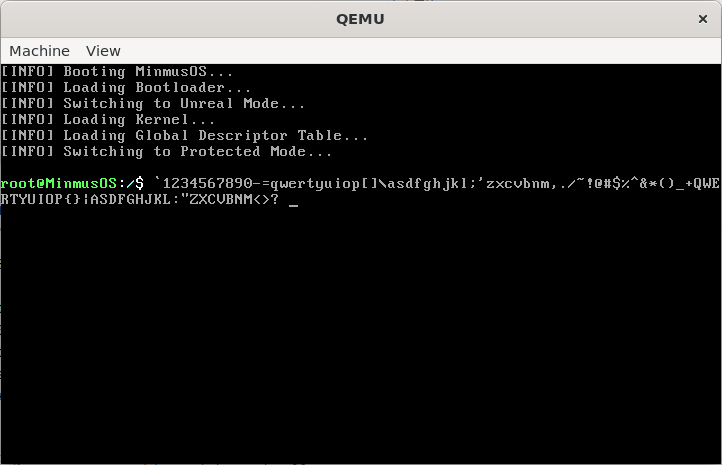
\includegraphics[width=0.8\textwidth]{figures/KeyboardDriverPresentation.png}
    \caption{键盘驱动程序演示}
    \label{fig:KeyboardDriverPresentation}
\end{figure}

\subsubsection{高级技术附件磁盘驱动程序(Advanced Technology Attachment Disk Driver)}

ATA(高级技术附件)磁盘驱动器是一种用于连接存储设备的标准接口,支持硬盘、软盘和光盘驱动器。虽然现代系统中更常见的是使用SATA接口,但ATA接口因其简单性在一些系统中仍被使用。

ATA磁盘驱动程序主要用于控制和管理磁盘读写操作。其核心功能之一是“读取”操作,该操作涉及以下几个步骤:

\begin{enumerate}
    \item \textbf{检查驱动器状态}:在进行读取之前,驱动程序会检查ATA驱动器是否启用并确保其处于非忙碌状态。
    \item \textbf{设置寄存器}:驱动程序设置ATA控制器的寄存器,输入必要的数据,如逻辑块地址(LBA)和要读取的扇区数量。
    \item \textbf{发送读取命令}:驱动程序向控制器发送读取命令,启动数据传输过程。
    \item \textbf{数据传输}:在读取命令发出后,控制器从磁盘读取数据到其内部缓冲区。驱动程序随后通过一个循环,从缓冲区将数据传输到指定的内存位置。由于磁盘的每个扇区大小通常为512字节,而缓冲区可能更小,例如4字节,因此需要多次迭代来完整地传输一个扇区的数据。
    \item \textbf{循环读取}:在每次迭代中,驱动程序都需要检查控制器是否已准备好下一次数据传输,确保不会在数据未完全就绪时进行读取。
\end{enumerate}

这种PIO(程序输入/输出)模式虽然对CPU负担较重,但由于其实现简单,因此在一些基础或旧的系统中仍然被采用。通过使用这种方法,ATA磁盘驱动程序能够有效地管理数据在存储设备与计算机内存之间的传输。

kernel/src/drivers/disk.rs 定义了一个高级技术附件磁盘驱动程序(Advanced Technology Attachment Disk Driver),这个磁盘驱动程序在实现上非常直接,主要通过直接与硬件寄存器交互来控制硬盘操作,而不依赖于操作系统提供的抽象层。

相关常量定义如下:

\begin{enumerate}
    \item \texttt{DATA\_REGISTER}:数据寄存器端口,用于读写数据。当进行数据传输时,数据会通过这个端口传入或传出。
    \item \texttt{SECTOR\_COUNT\_REGISTER}:扇区计数寄存器,用于指定在一个操作中要传输的扇区数量。
    \item \texttt{LBA\_LOW\_REGISTER}:LBA(逻辑块地址)的低位寄存器,用于指定LBA地址的低8位。
    \item \texttt{LBA\_MID\_REGISTER}:LBA(逻辑块地址)的中位寄存器,用于指定LBA地址的中8位。
    \item \texttt{LBA\_HIGH\_REGISTER}:LBA(逻辑块地址)的高位寄存器,用于指定LBA地址的高8位。
    \item \texttt{DRIVE\_REGISTER}:驱动器寄存器,用于选择操作的硬盘和该硬盘的哪个分区。
    \item \texttt{STATUS\_COMMAND\_REGISTER}:状态和命令寄存器。作为命令寄存器时用于发送命令给ATA控制器;作为状态寄存器时用于读取当前的设备状态。
    \item \texttt{READ\_COMMAND}:读取命令的代码,当要从硬盘读取数据时,通过状态命令寄存器发送这个命令。
    \item \texttt{STATUS\_BSY}:状态寄存器中的忙碌位标志,当硬盘忙碌时该位为1。
    \item \texttt{STATUS\_RDY}:状态寄存器中的就绪位标志,当硬盘准备好进行数据传输时该位为1。
\end{enumerate}

Disk 结构体定义了一个简单的 ATA 硬盘驱动程序,并包含多个方法用于硬盘的操作和状态检查。字段 enabled 类型为 bool,标识硬盘是否被启用。

\paragraph{is\_busy方法}

is\_busy 方法的主要功能是检查ATA硬盘的状态,确保在硬盘忙于处理其他命令时不会发起新的操作。这个方法通过查询硬盘的状态寄存器来判断是否有正在执行的任务,从而防止命令冲突和数据损坏。

\cref{lst:IsBusyMethod}使用 Rust 的内联汇编直接从硬盘的状态命令寄存器(STATUS\_COMMAND\_REGISTER)读取状态,特别关注忙碌位(BSY)。方法内部通过检查这个忙碌位是否设置(值为1),来确定硬盘是否处于忙碌状态,并返回相应的布尔值。这种直接与硬件寄存器交互的方式使得该方法既高效又精确。

\begin{listing}[htbp]
    \begin{minted}{rust}
pub fn is_busy(&self) -> bool {
    let status: u8;
    unsafe {
        asm!("in al, dx", out("al") status, in("dx") STATUS_COMMAND_REGISTER);
    }
    (status & STATUS_BSY) != 0
}
    \end{minted}
    \caption{is\_busy方法}\label{lst:IsBusyMethod}
\end{listing}

\paragraph{is\_ready方法}

is\_ready 方法的功能是检查ATA硬盘是否已经准备好接受新的命令。这个方法通过读取硬盘的状态寄存器来判断就绪位(RDY),如果就绪位被设置,表示硬盘处于空闲状态,可以安全地发送新的读写命令。

\cref{lst:IsReadyMethod}利用 Rust 的内联汇编语句从硬盘的状态命令寄存器(STATUS\_COMMAND\_REGISTER)直接读取状态值。方法通过检查就绪位(RDY),这个位在状态寄存器中的特定位置标识硬盘是否准备好进行操作。通过与就绪位掩码(STATUS\_RDY)进行按位与操作来确定硬盘是否就绪,如果结果为真,则返回 true,表示硬盘已经准备好接受新的操作。这种直接操作硬件寄存器的方法确保了检查的及时性和准确性。

\begin{listing}[htbp]
    \begin{minted}{rust}
pub fn is_ready(&self) -> bool {
    let status: u8;
    unsafe {
        asm!("in al, dx", out("al") status, in("dx") STATUS_COMMAND_REGISTER);
    }
    (status & STATUS_RDY) != 0
}
    \end{minted}
    \caption{is\_ready方法}\label{lst:IsReadyMethod}
\end{listing}

\paragraph{check方法}

check 方法的功能是验证ATA硬盘的操作状态,并更新硬盘的启用状态。此方法通过读取状态寄存器,检查硬盘是否正常响应命令,从而确定硬盘是否工作正常。如果状态寄存器的值表明硬盘处于异常状态(如完全不响应或返回错误状态),则硬盘将被标记为禁用。

\cref{lst:CheckMethod}使用 Rust 的内联汇编来直接从硬盘的状态命令寄存器读取当前状态值。通过判断这个状态值是否为 0 或 0xFF(通常表示硬件无响应或通信故障),来决定硬盘是否启用。如果状态值显示硬盘正常(即不是 0 或 0xFF),方法将 enabled 设置为 true 并记录信息日志;反之,设置为 false 并记录错误日志。这种方法可以及时捕捉到硬盘的异常状态,帮助进行故障诊断和维护。

\begin{listing}[htbp]
    \begin{minted}{rust}
pub fn check(&mut self) {
    let status: u8;
    unsafe {
        asm!("in al, dx", out("al") status, in("dx") STATUS_COMMAND_REGISTER);
    }
    if status != 0 && status != 0xFF {
        self.enabled = true;
        lib::println!("[INFO] ATA Disk Driver is Working. Status Register: 0x{:X}", status);
    } else {
        self.enabled = false;
        lib::println!("[ERROR] ATA Disk Driver is not Working! Status Register: 0x{:X}", status);
    }
}
    \end{minted}
    \caption{check方法}\label{lst:CheckMethod}
\end{listing}

\paragraph{reset方法}

reset 方法的主要功能是重置ATA硬盘,将其恢复到初始状态。这个操作对于解决硬盘冻结或响应异常的情况非常有用,通过发送特定的重置命令来清除任何挂起的操作或错误状态,确保硬盘能够重新开始接受命令。

\cref{lst:ResetMethod}通过 Rust 的内联汇编语句直接向硬盘的控制寄存器(位于端口 0x3F6)发送重置命令。具体地,它首先发送一个重置启动的命令(0b00000110),随后发送一个重置结束的命令(0b00000010)。这种直接与硬件寄存器交互的方式确保了命令的即时执行和硬盘状态的即时更新,从而有效地重置硬盘。

\begin{listing}[htbp]
    \begin{minted}{rust}
pub fn reset(&self) {
    unsafe {
        asm!("out dx, al", in("dx") 0x3F6, in("al") 0b00000110u8);
        asm!("out dx, al", in("dx") 0x3F6, in("al") 0b00000010u8);
    }
}
    \end{minted}
    \caption{reset方法}\label{lst:ResetMethod}
\end{listing}

\paragraph{read方法}

read 方法(\cref{lst:ReadMethod})的功能是从ATA硬盘上指定的逻辑块地址(LBA)开始读取一定数量的扇区数据到指定的内存地址。此方法在硬盘已启用且处于空闲状态时执行,通过设置必要的控制寄存器和发送读取命令,逐扇区地从硬盘读取数据并存储到提供的目标内存位置。该方法是硬盘驱动中实现数据读取的核心功能,确保了数据能够安全且有效地从硬盘传输到系统内存中。方法的实现逻辑如下:

\begin{enumerate}
    \item \textbf{检查硬盘是否启用}:方法首先检查 Disk 结构体的 enabled 字段。如果硬盘未启用,则输出错误信息并提前返回,不执行任何读取操作。
    \item \textbf{等待硬盘不忙}:在开始设置命令之前,方法循环调用 is\_busy 方法来确保硬盘不处于忙碌状态。这是必要的步骤,因为如果硬盘正忙于处理其他命令,尝试读取可能会导致命令失败或数据损坏。
    \item \textbf{设置控制寄存器}:使用内联汇编,方法设置了相关的控制寄存器来准备硬盘进行数据读取。
          \begin{enumerate}
              \item \textbf{扇区计数寄存器}:设置要读取的扇区数。
              \item \textbf{LBA 寄存器}:设置逻辑块地址,分为低、中、高位,确保完整的 LBA 地址被正确设置。
              \item \textbf{驱动器寄存器}:设置目标驱动器和LBA的最高位。
              \item \textbf{命令寄存器}:发送读取命令到硬盘。
          \end{enumerate}
    \item \textbf{读取数据}:初始化一个循环,根据指定的扇区数进行迭代。每个扇区通常是 512 字节。对于每个扇区,方法执行另一个循环128次(因为每次从数据寄存器读取4字节,512/4 = 128)。
          \begin{enumerate}
              \item 内部循环先检查硬盘是否忙碌,然后检查是否就绪。
              \item 使用内联汇编从数据寄存器读取4字节数据到本地变量 buffer。
              \item 使用 \texttt{core::ptr::write\_unaligned} 将读取的数据写入目标内存地址,并将目标指针移动4字节以准备下次写入。
          \end{enumerate}
    \item \textbf{重置硬盘}:在所有扇区读取完成后,调用 reset 方法将硬盘重置到初始状态,确保硬盘不会因为留下未完成的命令而出现问题。
\end{enumerate}

\begin{listing}[htbp]
    \begin{minted}{rust}
pub fn read<T>(&self, target: *mut T, lba: u64, sectors: u16) {
    if !self.enabled {
        lib::println!("[ERROR] Failed to Read Disk!");
        return;
    }

    while self.is_busy() {}

    unsafe {
        asm!("out dx, al", in("dx") 0x3F6, in("al") 0b00000010u8);
        asm!("out dx, al", in("dx") SECTOR_COUNT_REGISTER, in("al") sectors as u8);
        asm!("out dx, al", in("dx") LBA_LOW_REGISTER, in("al") lba as u8);
        asm!("out dx, al", in("dx") LBA_MID_REGISTER, in("al") (lba >> 8) as u8);
        asm!("out dx, al", in("dx") LBA_HIGH_REGISTER, in("al") (lba >> 16) as u8);
        asm!("out dx, al", in("dx") DRIVE_REGISTER, in("al") (0xE0 | ((lba >> 24) & 0xF)) as u8);
        asm!("out dx, al", in("dx") STATUS_COMMAND_REGISTER, in("al") READ_COMMAND);
    }

    let mut sectors_left = sectors;
    let mut target_pointer = target;

    while sectors_left > 0 {
        for _i in 0..128 {
            while self.is_busy() {}
            while !self.is_ready() {}
            let buffer: u32;
            unsafe {
                asm!("in eax, dx", out("eax") buffer, in("dx") DATA_REGISTER);
                core::ptr::write_unaligned(target_pointer as *mut u32, buffer);
                target_pointer = target_pointer.byte_add(4);
            }
        }
        sectors_left -= 1;
    }

    self.reset();
}
    \end{minted}
    \caption{read方法}\label{lst:ReadMethod}
\end{listing}

整个方法的实现逻辑既考虑了硬件操作的精确性,也确保了通过适当的检查和等待来避免硬件冲突。这种低级的硬盘操作需要精确控制硬件寄存器,同时确保数据的完整性和正确性。

\cref{fig:ATADiskDriverPresentation}展示了ATA磁盘驱动程序正在工作,且状态寄存器的值为 0x50。状态寄存器的值是一个 8 位的数,在硬盘接口中有特定的含义,每个位代表硬盘的一个不同的状态。对于状态寄存器值 0x50,将其转换为二进制表达为 0101 0000,分析如下:

\begin{enumerate}
    \item \textbf{位 7(BSY)}:0 - 硬盘当前不忙
    \item \textbf{位 6(DRDY)}:1 - 硬盘已准备好接受命令
    \item \textbf{位 5(DF)}:0 - 无设备故障
    \item \textbf{位 4(DSC)}:1 - 设备搜索操作已完成
    \item \textbf{位 3(DRQ)}:0 - 当前没有数据请求
    \item \textbf{位 2(CORR)}:0 - 无已纠正的数据
    \item \textbf{位 1(IDX)}:0 - 在检测到状态的时刻,磁盘的旋转周期没有重新开始
    \item \textbf{位 0(ERR)}:0 - 无错误
\end{enumerate}

\begin{figure}[htbp]
    \centering
    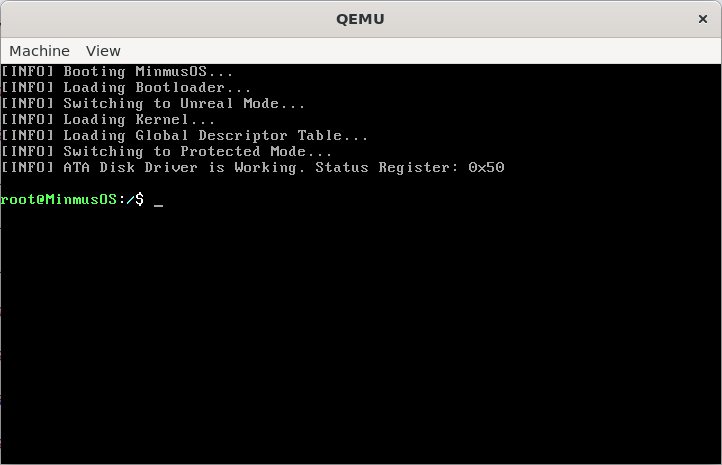
\includegraphics[width=0.8\textwidth]{figures/ATADiskDriverPresentation.png}
    \caption{ATA磁盘驱动程序演示}
    \label{fig:ATADiskDriverPresentation}
\end{figure}

\subsection{多任务处理(Multitasking)}

多任务处理是现代操作系统中一项基本功能,允许单个处理器同时运行多个任务。在单核系统中,虽然物理上不可能真正同时执行多个任务,但通过合理的时间分配,操作系统能够让用户感受到多个任务似乎是在同时运行。这种技术称为“并发”(Concurrency),它与真正的“并行”(Parallelism)不同,后者指的是在多核或多处理器系统中同时执行多个任务。

MinmusOS是一个支持抢占式多任务的操作系统。与协作式多任务系统不同,协作式系统中的任务需要主动放弃CPU使用权,抢占式系统则不需要任务主动放弃处理器。在抢占式系统中,操作系统通过定时器中断来强制从当前任务切换到另一个任务。每当定时器发送中断信号时,中断处理程序会调用调度程序,由调度程序决定下一个要执行的任务。这种方式确保了操作系统能高效地管理CPU资源,响应性好,可以处理大量任务,同时也增强了系统对于紧急处理需求的能力。

\subsubsection{上下文切换(Context Switching)}

在多任务操作系统中,上下文切换是一个至关重要的过程,它使得操作系统能够在多个任务之间高效切换,保证每个任务都能得到适当的处理器时间。上下文切换主要涉及保存当前任务的CPU状态,并在恢复执行另一个任务时加载其之前的状态。这样,即使任务被暂停,稍后恢复时也能如同从未停止过一样继续执行。

上下文的两个主要组成部分是任务栈(Task Stack)和CPU状态(CPU State):

\begin{enumerate}
    \item \textbf{任务栈}:每个任务都有自己的栈,这使得任务可以在需要时由调度器恢复。栈中保存着执行任务所需的所有信息,包括局部变量、函数调用的返回地址等。
    \item \textbf{CPU状态}:包括各种寄存器的值,如程序计数器、堆栈指针、状态寄存器等,这些寄存器的值决定了任务的执行状态。
\end{enumerate}

在 MinmusOS 中,定时器中断(IRQ9)负责在每个定时器滴答时触发调度程序。调度程序的一个关键指令是 mov esp, eax,这条指令将堆栈指针(ESP)设置为从定时器处理程序返回的值。该处理程序返回下一个要执行任务的堆栈指针。由于这个栈的底部包含了旧的CPU状态,所以弹出(popping)CPU寄存器就会恢复到该任务被暂停前的CPU状态。这种机制确保了操作系统能够在多个任务之间平滑且高效地切换,从而实现高度并发的执行,增强了系统的响应性和多任务处理能力。

\cref{lst:TimerFunction}使用了裸函数(\texttt{\#[naked]}),这意味着该函数不会由编译器生成入口和退出代码,完全依赖于程序员手写的汇编代码来控制。这是必须的,因为上下文切换需要精确地控制栈和寄存器的状态。

\begin{listing}[htbp]
    \begin{minted}{rust}
#[naked]
pub extern "C" fn timer() {
    unsafe {
        core::arch::asm!(
        "cli",                // 禁用中断,确保上下文切换不被打断
        "push ebp",           // 保存所有寄存器,以保持当前任务的状态
        "push edi",
        "push esi",
        "push edx",
        "push ecx",
        "push ebx",
        "push eax",
        "push esp",           // 将当前栈指针(esp)压栈,作为参数传递给 C 函数
        "call timer_handler", // 调用 Rust 部分的处理函数
        "mov esp, eax",       // 将 C 函数返回的新栈指针设为当前栈指针
        "pop eax",            // 恢复所有寄存器
        "pop ebx",
        "pop ecx",
        "pop edx",
        "pop esi",
        "pop edi",
        "pop ebp",
        "sti",                // 重新开启中断
        "iretd",              // 从中断返回
        options(noreturn),
        );
    }
}
    \end{minted}
    \caption{timer函数}\label{lst:TimerFunction}
\end{listing}

\cref{lst:TimerHandlerFunction}是上下文切换逻辑的核心。在 timer\_handler 函数中,上下文切换的实现涉及调用任务调度器以选择下一个执行的任务并获取其栈指针,计算该任务在内存中的目标地址,然后更新页表以映射到新的任务地址。这样,当中断处理完成后,CPU可以从新任务的保存状态继续执行,实现任务间的无缝切换。

\begin{listing}[htbp]
    \begin{minted}{rust}
#[no_mangle]
pub extern "C" fn timer_handler(esp: u32) -> u32 {
    unsafe {
        // 调用任务调度器,并传递当前的栈指针,返回新任务的栈指针
        let new_esp: u32 = TASK_MANAGER.schedule(esp as *mut CPUState) as u32;
        // 获取当前任务的槽位
        let slot = TASK_MANAGER.get_current_slot();
        // 计算当前任务的内存目标地址
        let target = APP_TARGET + (slot as u32 * APP_SIZE);
        // 更新页表,将任务的代码映射到正确内存位置,确保 CPU 在执行新任务时访问到正确的代码和数据
        TABLES[8].set(target);
        // 使页表更改生效
        PAGING.set_table(8, &TABLES[8]);
        // 发送中断结束信号到 PIC,告知中断处理完成
        PICS.end_interrupt(TIMER_INT);
        // 返回新的栈指针
        new_esp
    }
}
    \end{minted}
    \caption{timer\_handler函数}\label{lst:TimerHandlerFunction}
\end{listing}

这种结合汇编和高级语言的方式允许操作系统精确控制硬件,实现高效的多任务处理和上下文切换。通过这样的实现,即使在单核处理器上,操作系统也能够提供平滑的多任务环境。

\subsubsection{CPU 调度器(CPU Scheduler)}\label{sec:CPUScheduler}

MinmusOS 使用了轮转调度(round robin)算法来管理任务的调度,该算法通过定时器中断处理程序触发。每当发生一个定时器滴答,调度算法就会从任务列表中选择下一个任务,并返回一个指向该任务CPU状态的指针。

这个返回的指针非常关键,因为它指向了被选择任务的CPU状态。在上下文切换时,上下文切换器会将栈指针设置为这个指针,并从中弹出(pop)寄存器的值,以此恢复任务的状态。这样,当任务再次运行时,就可以从上次停止的地方继续执行,实现任务间的平滑切换。

轮转调度(Round Robin, RR)算法是一种非常常见的任务调度方法,尤其适用于时间分片的操作系统中。在RR算法中,每个任务被赋予一个固定时间的时间片或量子(quantum),所有任务按照一定的顺序排列,形成一个循环队列。

轮转调度算法的主要特点和步骤包括:

\begin{enumerate}
    \item \textbf{时间片}:系统为每个任务分配一个固定长度的时间片,这是任务可以连续运行的最大时间。时间片的长度通常由操作系统确定,需要平衡响应时间和系统效率。
    \item \textbf{任务切换}:当一个任务的时间片用完时,如果它还没有完成,则会被操作系统挂起。调度器将CPU控制权转移给队列中的下一个任务。
    \item \textbf{循环队列}:所有等待运行的任务形成一个循环队列。调度器按照队列的顺序为每个任务分配CPU时间,一旦到达队列末尾,调度器就从队列头开始新一轮的任务调度。
    \item \textbf{公平性}:RR算法的一个显著优点是它的公平性。每个任务都有相同长度的时间运行,这意味着没有单个任务能长时间独占CPU,从而保证了所有任务都能获得足够的处理时间。
    \item \textbf{响应时间}:由于任务经常被切换,RR算法能提供较好的响应时间,适合需要频繁交互的应用。但是,频繁的任务切换也可能导致较高的开销,因为每次切换都需要进行上下文保存和恢复。
\end{enumerate}

轮转调度算法适用于多任务环境,尤其是处理许多短任务的系统。通过合理设置时间片长度,可以使系统达到良好的性能平衡。

\begin{listing}[htbp]
    \begin{minted}{rust}
pub fn schedule(&mut self, cpu_state: *mut CPUState) -> *mut CPUState {
    if self.task_count <= 0 {
        return cpu_state;
    }
    if self.current_task >= 0 {
        self.tasks[self.current_task as usize].cpu_state_ptr = cpu_state as u32;
    }
    self.current_task = self.get_next_task();
    self.tasks[self.current_task as usize].cpu_state_ptr as *mut CPUState
}

pub fn get_next_task(&self) -> i8 {
    let mut i = self.current_task + 1;
    while i < MAX_TASKS {
        if self.tasks[i as usize].running {
            return i;
        }
        i = (i + 1) % MAX_TASKS;
    }
    -1
}
    \end{minted}
    \caption{轮转调度(Round Robin, RR)算法}\label{lst:RoundRobinAlgorithm}
\end{listing}

\cref{lst:RoundRobinAlgorithm}通过两个主要函数 schedule 和 get\_next\_task 来实现轮转调度算法。schedule 函数首先检查是否有任务在运行,如果有,它会保存当前任务的CPU状态。然后,它调用 get\_next\_task 函数,从任务列表中按顺序选择下一个可运行的任务,并返回该任务的CPU状态指针,供系统加载和执行。

get\_next\_task 函数实现了任务的轮转选择逻辑。它从当前任务的下一个任务开始查找,直到找到一个正在运行的任务。如果到达任务列表末尾,它会循环回到列表的开头,继续查找。如果找不到任何运行的任务,则返回 -1。

这种实现方式确保了所有任务都能依次得到执行机会,公平地分配CPU时间,符合轮转调度算法的特点。

\subsubsection{任务管理器(Task Manager)}

任务管理器(Task Manager)是操作系统中负责管理任务的组件,主要职责包括插入、移除和调度任务。任务管理器由多个函数组成,用于操作任务列表,并包含一个数据结构,存储任务数组、任务数量以及当前正在运行任务的ID。

\paragraph{\texttt{CPUState}数据结构}

CPUState 是一个表示 CPU 状态的结构体(\cref{lst:CPUStateDataStructure}),使用 \texttt{\#[repr(C, packed)]} 属性确保其在内存中的布局与 C 语言的结构体一致且紧密排列。这个结构体保存了寄存器的状态,其中包括手动压入栈的寄存器(如 eax, ebx, ecx, edx, esi, edi, ebp)和 CPU 自动压入的寄存器(如 eip, cs, eflags, esp, ss)。这些寄存器的值通常在上下文切换或异常处理中被保存和恢复,以确保线程或异常处理返回时能够继续正确的执行。

\begin{listing}[htbp]
    \begin{minted}{rust}
#[repr(C, packed)]
pub struct CPUState {
    eax: u32,
    ebx: u32,
    ecx: u32,
    edx: u32,
    esi: u32,
    edi: u32,
    ebp: u32,
    eip: u32,
    cs: u32,
    eflags: u32,
    esp: u32,
    ss: u32,
}
    \end{minted}
    \caption{\texttt{CPUState}数据结构}\label{lst:CPUStateDataStructure}
\end{listing}

\paragraph{\texttt{Task}数据结构}

Task 结构体(\cref{lst:TaskDataStructure})表示操作系统中的一个任务。它包含了任务运行所需的关键信息,包括一个固定大小的栈 stack,一个指向 CPU 状态保存位置的指针 cpu\_state\_ptr,以及一个布尔值 running,用于表示任务是否正在运行。stack 用于存储任务的局部变量和函数调用信息,而 cpu\_state\_ptr 指向 CPUState 结构体,以保存任务的寄存器状态,方便在任务切换时进行恢复。

\begin{listing}[htbp]
    \begin{minted}{rust}
#[derive(Copy, Clone, Debug)]
pub struct Task {
    pub stack: [u8; STACK_SIZE],
    pub cpu_state_ptr: u32,
    pub running: bool,
}

impl Task {
    pub fn init(&mut self, entry_point: u32) {
        self.running = true;
        let mut state = &self.stack as *const u8;
        unsafe {
            state = state.byte_add(STACK_SIZE);
            state = state.byte_sub(size_of::<CPUState>());
        }
        self.cpu_state_ptr = state as u32;
        let cpu_state = self.cpu_state_ptr as *mut CPUState;
        unsafe {
            (*cpu_state).eax = 0;
            (*cpu_state).ebx = 0;
            (*cpu_state).ecx = 0;
            (*cpu_state).edx = 0;
            (*cpu_state).esi = 0;
            (*cpu_state).edi = 0;
            (*cpu_state).ebp = 0;
            (*cpu_state).eip = entry_point;
            (*cpu_state).cs = 0x8;
            (*cpu_state).eflags = 0x202;
        }
    }
}
    \end{minted}
    \caption{\texttt{Task}数据结构}\label{lst:TaskDataStructure}
\end{listing}

Task 结构体实现了一个 init 方法,用于初始化任务。初始化过程中,将 running 标记为 true,表示任务开始运行。然后计算 CPUState 的位置,cpu\_state\_ptr 指向栈顶减去 CPUState 大小的位置,确保 CPUState 有足够的空间存储在栈中。接着,初始化 CPUState 结构体中的各个寄存器值:

\begin{enumerate}
    \item \textbf{通用寄存器(eax, ebx, ecx, edx, esi, edi, ebp)}:设置为 0,以保证任务开始时寄存器处于已知状态。
    \item \textbf{程序计数器(eip)}:设置为传入的 entry\_point,表示任务从这个地址开始执行。entry\_point 是任务的入口地址,通常指向任务的第一条指令。
    \item \textbf{代码段寄存器(cs)}:设置为 0x8,这是一个常见的代码段选择子,通常在操作系统中表示内核代码段。
    \item \textbf{标志寄存器(eflags)}:设置为 0x202。0x202 表示启用了中断(IF 位为 1),并且设置了固定的保留位。这样可以确保任务在开始执行时,CPU的标志状态正确。
\end{enumerate}

NULL\_TASK 是一个静态变量(\cref{lst:NullTaskStaticVariable}),用作任务的默认空白模板,表示未初始化或未运行的任务。它的 stack 被初始化为全零,cpu\_state\_ptr 为 0,running 标志设置为 false。NULL\_TASK 在创建新任务时作为基础,并通过调用 init 方法进行具体的初始化,避免每次创建任务时都手动构建任务结构体。

\begin{listing}[htbp]
    \begin{minted}{rust}
static NULL_TASK: Task = Task {
    stack: [0; STACK_SIZE],
    cpu_state_ptr: 0u32,
    running: false,
};
    \end{minted}
    \caption{NULL\_TASK静态变量}\label{lst:NullTaskStaticVariable}
\end{listing}

\paragraph{\texttt{TaskManager}数据结构}

TaskManager 是一个管理操作系统中所有任务的结构体(\cref{lst:TaskManagerDataStructure})。它包含以下几个重要字段:

\begin{enumerate}
    \item \texttt{tasks}:一个固定大小的数组,用于存储系统中的所有任务。数组的大小由常量 MAX\_TASKS 决定,每个元素都是一个 Task 结构体实例。
    \item \texttt{task\_count}:记录当前运行的任务数量。
    \item \texttt{current\_task}:表示当前正在执行的任务的索引。使用 -1 表示没有当前任务或系统处于空闲状态。
\end{enumerate}

\begin{listing}[htbp]
    \begin{minted}{rust}
pub struct TaskManager {
    pub(crate) tasks: [Task; MAX_TASKS as usize],
    task_count: i8,
    current_task: i8,
}

impl TaskManager {
    pub fn init(&mut self) {
        self.add_task(idle as u32);
    }

    pub fn add_task(&mut self, entry_point: u32) {
        self.tasks[self.get_free_slot() as usize].init(entry_point);
        self.task_count += 1;
    }

    pub fn remove_task(&mut self, id: usize) {
        if id != 0 {
            self.tasks[id] = NULL_TASK;
            self.task_count -= 1;
        }
    }

    pub fn remove_current_task(&mut self) {
        self.remove_task(self.current_task as usize);
    }

    pub fn schedule(&mut self, cpu_state: *mut CPUState) -> *mut CPUState { ... }

    pub fn get_next_task(&self) -> i8 { ... }

    pub fn get_free_slot(&self) -> i8 {
        let mut slot: i8 = -1;
        for i in 0..MAX_TASKS {
            if self.tasks[i as usize].running == false {
                slot = i;
                return slot;
            }
        }
        slot
    }

    pub fn get_current_slot(&self) -> i8 {
        self.current_task
    }

    pub fn list_tasks(&self) {
        lib::println!("Running tasks:");
        for i in 0..MAX_TASKS {
            if self.tasks[i as usize].running {
                lib::println!("PID: {}", i);
            }
        }
    }
}
    \end{minted}
    \caption{\texttt{TaskManager}数据结构}\label{lst:TaskManagerDataStructure}
\end{listing}

TaskManager 的方法实现如下:

\begin{enumerate}
    \item \texttt{init}:添加一个空闲任务(idle),以确保即使没有其他任务运行,系统也有一个默认任务执行。idle 函数是一个空闲任务,在一个无限循环中执行 hlt 指令,以使 CPU 进入低功耗状态,等待外部中断恢复。
    \item \texttt{add\_task}:向任务管理器中添加一个新任务。它会先找到一个空闲的任务槽(未使用的 Task 实例),然后初始化该任务,并将 task\_count 计数器加 1。
    \item \texttt{remove\_task}:删除指定 ID 的任务。该方法会重置任务槽为 NULL\_TASK,并减少任务数量。
    \item \texttt{remove\_current\_task}:删除当前正在运行的任务。它调用 remove\_task 方法,并传入当前任务的 ID。
    \item \texttt{schedule}和\texttt{get\_next\_task}:通过轮转调度算法进行任务调度。保存当前任务的 CPU 状态,然后选择下一个任务并返回其 CPU 状态指针,具体实现见\cref{sec:CPUScheduler},在此不再赘述。
    \item \texttt{get\_free\_slot}:找到第一个空闲任务槽的索引。如果没有找到空闲槽,返回 -1。
    \item \texttt{get\_current\_slot}:返回当前正在运行的任务的索引。
    \item \texttt{list\_tasks}:列出所有正在运行的任务的 PID。
\end{enumerate}

TASK\_MANAGER 静态变量(\cref{lst:TaskManagerStaticVariable})是整个操作系统中唯一的 TaskManager 实例,用于全局管理所有的任务。它的作用包括:

\begin{listing}[htbp]
    \begin{minted}{rust}
pub static mut TASK_MANAGER: TaskManager = TaskManager {
    tasks: [NULL_TASK; MAX_TASKS as usize],
    task_count: 0,
    current_task: -1,
};
    \end{minted}
    \caption{TASK\_MANAGER静态变量}\label{lst:TaskManagerStaticVariable}
\end{listing}

\begin{enumerate}
    \item \textbf{任务管理的核心控制}:跟踪和调度系统中的所有任务。它持有任务列表(tasks),管理当前任务的状态(current\_task),并记录系统中总共存在的任务数量(task\_count)。
    \item \textbf{提供全局访问}:系统中各个部分可以方便地访问这个任务管理器,这对于任务调度、任务创建、删除、切换等操作非常重要。
    \item \textbf{任务初始化和调度}:在系统启动时初始化默认任务(例如 idle 任务),并在系统运行过程中负责调度各个任务。这使得操作系统能够在多任务环境下正确地进行任务切换,确保系统的稳定运行。
    \item \textbf{持久存在的状态管理}:作为静态变量,TASK\_MANAGER 的生命周期贯穿整个系统的运行期,它的状态在整个操作系统运行过程中是持久的。这意味着任务的状态不会在函数调用结束时丢失,可以在任意时间点被访问和修改。
\end{enumerate}

\subsection{系统调用(System Calls)}

\subsubsection{系统调用概述}

在MinmusOS中,kernel/src/syscalls/handler.rs文件(\cref{lst:HandlerRust})负责处理系统调用。系统调用是用户空间中的程序请求内核服务的一种方式。通过这个接口,内核可以建立一个安全模型,对某些进程可以执行的操作类型和范围进行限制,它是内核功能对用户空间的一种暴露。

在MinmusOS中,系统调用通过\texttt{syscall()}函数使用软件中断(中断向量0x80)来触发。这种机制类似于Linux在x86架构上使用的方法。

目前,MinmusOS只支持两个系统调用:

\begin{enumerate}
    \item \textbf{系统调用0}:打印由EBX寄存器指向的地址开始的字符串,长度由ECX寄存器指定。
    \item \textbf{系统调用1}:从任务列表中移除当前运行的任务。
\end{enumerate}

\subsubsection{系统调用实现}

以下是处理系统调用的关键步骤:

\begin{enumerate}
    \item \textbf{中断触发和保存寄存器}:使用\texttt{asm!}宏定义的\texttt{syscall()}函数负责保存寄存器状态并调用\texttt{syscall\_handler()}函数。这里eax,ebx和ecx寄存器被推入堆栈,并在调用完\texttt{syscall\_handler}之后恢复,最后执行\texttt{iretd}从中断返回。在\texttt{syscall()}函数中,eax,ebx和ecx寄存器的值被依次推入栈中,每个寄存器都是32位,即4字节。所以,总共推入了12字节。函数执行结束后,需要将这些值从栈上移除,以恢复调用前的栈状态。这就是\texttt{add esp, 12}的作用:它通过增加esp的值来“弹出”这些值,即将栈指针向上移动12字节,回到调用\texttt{syscall\_handler}函数之前的位置。
    \item \textbf{处理系统调用}:\texttt{syscall\_handler()}函数接收来自eax,ebx和ecx寄存器的值作为参数,这些寄存器在\texttt{syscall()}中被传递。eax用于指定系统调用的类型,ebx和ecx用于传递额外的参数或数据。
    \item \textbf{系统调用的分发}:通过检查eax寄存器的值来确定要执行的具体系统调用。
          \begin{enumerate}
              \item \textbf{系统调用0}:打印字符串。通过ebx寄存器传递的地址读取字符串,ecx指定字符串的长度。使用Rust的\texttt{slice::from\_raw\_parts()}和\texttt{str::from\_utf8()}将字节转换为字符串。
              \item \textbf{系统调用1}:移除当前活动任务,通过调用任务管理器的\texttt{remove\_current\_task()}方法来实现。
          \end{enumerate}
    \item \textbf{结束中断处理}:调用\texttt{PICS.end\_interrupt()}方法,标志着对此次中断的处理已经完成,可以继续执行其他操作。
\end{enumerate}

\begin{listing}[htbp]
    \begin{minted}{rust}
#[naked]
pub extern "C" fn syscall() {
    unsafe {
        asm!(
        "push eax",
        "push ebx",
        "push ecx",
        "call syscall_handler",
        "add esp, 12",
        "iretd",
        options(noreturn),
        );
    }
}

#[no_mangle]
pub extern "C" fn syscall_handler(ecx: u32, ebx: u32, eax: u32) {
    unsafe {
        match eax {
            0 => {
                let s = {
                    let slice = slice::from_raw_parts(ebx as *const u8, ecx as usize);
                    str::from_utf8(slice)
                };
                print::PRINTER.prints(s.unwrap());
            }
            1 => {
                TASK_MANAGER.remove_current_task();
            }
            _ => {}
        }
        PICS.end_interrupt(SYSCALL_INT);
    }
}
    \end{minted}
    \caption{kernel/src/syscalls/handler.rs}\label{lst:HandlerRust}
\end{listing}

通过这种方式,MinmusOS能够提供一种有效且安全的机制,允许用户程序执行核心级的操作,如IO操作和任务管理。

\subsection{VGA文本模式(VGA Text Mode)}

VGA文本模式是VGA标准的一种模式,专门用于显示标准的文本字符而非图形。这种模式通常用于计算机启动过程中和一些基本的用户界面,因为它可以提供快速且低消耗的文本显示功能。

在VGA文本模式中,屏幕通常被分成一个个字符单元,每个字符单元可以显示一个字符。常见的配置是80列和25行,即屏幕上可以同时显示2000个字符。每个字符单元由一个字符码和一个属性码组成,字符码用来确定显示哪个字符,属性码定义了字符的前景色和背景色以及是否闪烁等属性。

VGA文本模式支持ASCII字符集的扩展,包括英文字符和各种符号,以及一些特殊的图形符号,这使得它能够用来绘制简单的图形和边框。由于其简洁和高效的特性,VGA文本模式在早期的个人计算机和一些嵌入式系统中得到了广泛使用。

\subsubsection{标准色彩定义}

在VGA文本模式中,标准色彩定义为前景色和背景色的组合,从而在文本显示中实现不同的视觉效果。如\cref{lst:StandardColorDefinitions}所示,我们定义了一系列的颜色常量,包括基本的黑色、蓝色、绿色、红色等,以及它们的“亮”版本,如亮黑色、亮蓝色等。这些颜色常量使用一个无符号8位整数(u8)表示,其中每个颜色对应一个唯一的数值,例如黑色为0,蓝色为1等。

这些颜色可以在VGA文本模式下用于设置字符的前景色和背景色。在设置字符属性时,前景色和背景色的值可以通过位操作组合在一起,其中背景色占高四位,前景色占低四位。这种色彩配置方法允许快速和简单地调整文本的视觉样式,是文本模式下高效显示的关键。

\begin{listing}[htbp]
    \begin{minted}{rust}
pub const COLOR_BLACK: u8 = 0x0;
pub const COLOR_BLUE: u8 = 0x1;
pub const COLOR_GREEN: u8 = 0x2;
pub const COLOR_CYAN: u8 = 0x3;
pub const COLOR_RED: u8 = 0x4;
pub const COLOR_MAGENTA: u8 = 0x5;
pub const COLOR_YELLOW: u8 = 0x6;
pub const COLOR_WHITE: u8 = 0x7;
pub const COLOR_LIGHT_BLACK: u8 = 0x8;
pub const COLOR_LIGHT_BLUE: u8 = 0x9;
pub const COLOR_LIGHT_GREEN: u8 = 0xA;
pub const COLOR_LIGHT_CYAN: u8 = 0xB;
pub const COLOR_LIGHT_RED: u8 = 0xC;
pub const COLOR_LIGHT_MAGENTA: u8 = 0xD;
pub const COLOR_LIGHT_YELLOW: u8 = 0xE;
pub const COLOR_LIGHT_WHITE: u8 = 0xF;
    \end{minted}
    \caption{标准色彩定义}\label{lst:StandardColorDefinitions}
\end{listing}

\subsubsection{printc方法}

printc方法(\cref{lst:PrintcMethod})是VGA文本模式中用于在屏幕上打印单个字符的函数。该方法接受一个字符参数,并根据当前光标位置将字符显示在屏幕上。在VGA文本模式中,屏幕被视为一个由多个字符单元组成的数组,每个单元可以显示一个字符和相应的颜色属性。

该方法首先检查传入的字符是否为换行符。如果是,它将调用new\_line方法来移动到下一行。如果不是换行符,方法将计算当前字符应该放置的内存位置。这个位置由VGA\_START(VGA内存的起始地址)加上基于当前行(self.y)和列(self.x)的偏移量计算得出。每个字符单元占用两个字节:第一个字节用于存储字符的ASCII码,第二个字节用于存储该字符的颜色属性(由前景色和背景色组成)。

方法中还包含了对屏幕边界的检查。如果字符位置达到屏幕的最右侧或最下方,它会通过调用scroll方法来滚动屏幕内容,为新字符腾出空间。每打印一个字符后,方法会通过调用set\_cursor\_position更新光标位置,确保下一个字符能够被正确打印。

\begin{listing}[htbp]
    \begin{minted}{rust}
pub fn printc(&mut self, c: char) {
    if c == '\n' {
        self.new_line();
        return;
    }
    let target: *mut u8 = (VGA_START + ((self.y * VGA_WIDTH + self.x) * 2) as u32) as *mut u8;
    unsafe {
        if self.y >= VGA_HEIGHT - 1 && self.x >= VGA_WIDTH - 1 {
            *target = c as u8;
            *target.byte_add(1) = self.bg_color << 4 | self.fg_color;
            self.scroll();
            self.x = 0;
        } else {
            *target = c as u8;
            *target.byte_add(1) = self.bg_color << 4 | self.fg_color;
            self.x += 1;
            if self.x >= VGA_WIDTH {
                self.x = 0;
                self.y += 1;
            }
        }
    }
    self.set_cursor_position();
}
    \end{minted}
    \caption{printc方法}\label{lst:PrintcMethod}
\end{listing}

\subsubsection{prints方法}

prints方法(\cref{lst:PrintsMethod})用于在VGA文本模式中打印一个字符串。此方法接受一个字符串参数,并逐字符调用printc方法将字符串的每个字符输出到屏幕上。

首先,此方法通过调用get\_cursor\_position获取当前光标的位置,确保字符串从正确的位置开始打印。光标位置以(u16, u16)格式返回,表示当前光标的行(y)和列(x)。获取到这个位置后,方法将此位置赋值给内部的x和y属性,从而准备字符打印的起始点。

接着,方法遍历字符串中的每一个字符,并逐个调用printc方法进行打印。由于printc方法已经内置了处理换行和屏幕滚动的逻辑,prints方法可以无缝地继续打印字符串,即使内容跨越多行。

在字符串的所有字符都被打印后,prints方法会再次调用set\_cursor\_position以更新屏幕的光标位置,确保后续的输出能够从正确的位置开始。通过这种方式,prints方法提供了一种高效且方便的方式来在VGA文本模式下输出完整的字符串。

\begin{listing}[htbp]
    \begin{minted}{rust}
pub fn prints(&mut self, s: &str) {
    let cursor: (u16, u16) = self.get_cursor_position();
    self.x = cursor.0;
    self.y = cursor.1;
    for c in s.chars() {
        self.printc(c);
    }
    self.set_cursor_position();
}
    \end{minted}
    \caption{prints方法}\label{lst:PrintsMethod}
\end{listing}

\subsubsection{delete方法}

delete 方法(\cref{lst:DeleteMethod})在 VGA 文本模式中的实现允许用户擦除屏幕上最后一个显示的字符。此方法通过检查当前光标位置并适当调整,以定位需要擦除的字符。如果光标不在行首,它将向左移动一个位置;如果在行首但非屏幕顶端,则移动到上一行的末尾。接着,方法在计算出的地址位置写入空格字符,实际上是用空格覆盖了原字符,同时保持字符的颜色属性不变。这个过程不仅包括了字符的视觉擦除,也正确地更新了光标的位置,确保了继续输入或进一步删除的准确性。

\begin{listing}[htbp]
    \begin{minted}{rust}
pub fn delete(&mut self) {
    if self.x > 0 {
        self.x -= 1;
    } else if self.y > 0 {
        self.y -= 1;
        self.x = VGA_WIDTH - 1;
    } else {
        return;
    }
    let target: *mut u8 = (VGA_START + ((self.y * VGA_WIDTH + self.x) * 2) as u32) as *mut u8;
    unsafe {
        *target = b' ' as u8;
        *target.byte_add(1) = self.bg_color << 4 | self.fg_color;
    }
    self.set_cursor_position();
}
    \end{minted}
    \caption{delete方法}\label{lst:DeleteMethod}
\end{listing}

\subsubsection{get\_cursor\_position方法}

get\_cursor\_position 方法(\cref{lst:GetCursorPositionMethod})在 VGA 文本模式中用于获取当前光标的位置。此方法是理解和操作光标在屏幕上的位置的关键,它返回一个包含两个元素的元组 (u16, u16),分别代表光标的列(x 坐标)和行(y 坐标)。

该方法的实现涉及到对硬件端口的直接操作,以查询视频硬件当前的光标位置。具体步骤如下:

\begin{enumerate}
    \item \textbf{初始化变量}:方法开始时,初始化一个用于存储光标位置索引的变量 index。
    \item \textbf{读取光标低字节}:通过向 VGA 控制寄存器(端口 0x3D4)写入命令 0x0F,请求返回光标位置的低字节。随后从数据寄存器(端口 0x3D5)读取这个字节并存入 index。
    \item \textbf{读取光标高字节}:再次向控制寄存器写入命令 0x0E,请求返回光标位置的高字节。读取该字节后,将其左移8位并与 index 合并,从而得到完整的光标位置索引。
    \item \textbf{计算坐标}:使用 index 值计算光标的行和列坐标。光标的列坐标是 index \% VGA\_WIDTH(index 与屏幕宽度的余数),行坐标是 index / VGA\_WIDTH(index 除以屏幕宽度的商)。
\end{enumerate}

通过这种方法,get\_cursor\_position 函数能够准确地从底层硬件中检索光标的当前位置,为屏幕上的文本操作提供必要的坐标信息。

\begin{listing}[htbp]
    \begin{minted}{rust}
pub fn get_cursor_position(&self) -> (u16, u16) {
    let mut index: u16 = 0;
    unsafe {
        asm!("out dx, al", in("dx") 0x3D4u16, in("al") 0x0Fu8);
        let mut a: u8;
        asm!("in al, dx", out("al") a, in("dx") 0x3D5);
        index |= a as u16;
        asm!("out dx, al", in("dx") 0x3D4u16, in("al") 0x0Eu8);
        let b: u8;
        asm!("in al, dx", out("al") b, in("dx") 0x3D5);
        index |= (b as u16) << 8;
    }
    (index % VGA_WIDTH, index / VGA_WIDTH)
}
    \end{minted}
    \caption{get\_cursor\_position方法}\label{lst:GetCursorPositionMethod}
\end{listing}

\subsubsection{set\_cursor\_position方法}

set\_cursor\_position 方法(\cref{lst:SetCursorPositionMethod})在 VGA 文本模式中用于设置光标的位置。此方法是调整屏幕上光标位置的关键函数,确保文本输入和编辑能够在正确的屏幕位置进行。它通过直接与硬件通信,将光标定位到由内部状态(self.x 和 self.y)指定的新位置。

该方法的执行过程涉及以下步骤:

\begin{enumerate}
    \item \textbf{计算光标索引}:首先,根据光标的行 (self.y) 和列 (self.x) 坐标,计算光标在 VGA 文本缓冲区中的线性位置索引。这是通过表达式 self.y * VGA\_WIDTH + self.x 完成的,其中 VGA\_WIDTH 是屏幕的宽度(通常为80个字符)。
    \item \textbf{设置光标低字节}:使用汇编指令向 VGA 控制寄存器(端口 0x3D4)写入光标位置低字节的命令 0x0F,然后通过数据寄存器(端口 0x3D5)设置光标位置的低字节,即 index \& 0xFF(索引的低8位)。
    \item \textbf{设置光标高字节}:继续使用汇编指令向 VGA 控制寄存器写入光标位置高字节的命令 0x0E,再通过数据寄存器设置光标位置的高字节,即 (index >> 8) \& 0xFF(索引的高8位)。
\end{enumerate}

通过这种方法,set\_cursor\_position 函数能够精确地将光标移动到所需的屏幕位置,这对于实现屏幕文本的正确渲染和用户交互的流畅性是至关重要的。

\begin{listing}[htbp]
    \begin{minted}{rust}
pub fn set_cursor_position(&self) {
    let index: u16 = self.y * VGA_WIDTH + self.x;
    unsafe {
        asm!("out dx, al", in("dx") 0x3D4u16, in("al") 0x0Fu8);
        asm!("out dx, al", in("dx") 0x3D5u16, in("al") (index & 0xFF) as u8);
        asm!("out dx, al", in("dx") 0x3D4u16, in("al") 0x0Eu8);
        asm!("out dx, al", in("dx") 0x3D5u16, in("al") ((index >> 8) & 0xFF) as u8);
    }
}
    \end{minted}
    \caption{set\_cursor\_position方法}\label{lst:SetCursorPositionMethod}
\end{listing}

\subsubsection{scroll方法}

scroll 方法(\cref{lst:ScrollMethod})在 VGA 文本模式中用于滚动屏幕内容,使得当文本到达屏幕底部时可以继续显示新的文本。这个方法是文本模式下管理屏幕输出的重要组成部分,尤其是在处理长文本或连续输出时非常有用。

该方法的基本逻辑如下:

\begin{enumerate}
    \item \textbf{内存复制}:方法首先遍历屏幕上的每一行。对于每一行,它计算当前行在 VGA 内存中的起始地址,并将其上一行的内容复制到当前行的位置。这种操作实质上是将屏幕上所有行的内容向上移动一行。
    \item \textbf{处理最后一行}:由于最顶部的一行被移出屏幕,最底部的新行需要被清空或用新的内容填充。在此实现中,新的行通常会被清空或设置为默认的背景和前景色,以等待新的文本输入。
    \item \textbf{内存操作安全性}:所有内存操作都是在 unsafe 块中执行的,因为它们涉及直接的指针操作。这是必要的,因为 VGA 文本模式直接与硬件相关的内存交互,需要确保操作的正确性和内存安全。
\end{enumerate}

通过这种方式,scroll 方法有效地管理了屏幕空间,确保即使在连续输出的情况下也能保持屏幕内容的连续性和可读性。

\begin{listing}[htbp]
    \begin{minted}{rust}
pub fn scroll(&mut self) {
    for i in 0..VGA_HEIGHT {
        for j in (VGA_WIDTH * i)..((VGA_WIDTH * i) + VGA_WIDTH) {
            let new: *mut u8 = (VGA_START + (j * 2) as u32) as *mut u8;
            let old: *const u8 = (VGA_START + ((j + VGA_WIDTH) * 2) as u32) as *const u8;
            unsafe {
                *new = *old;
                *new.byte_add(1) = *old.byte_add(1);
            }
        }
    }
}
    \end{minted}
    \caption{scroll方法}\label{lst:ScrollMethod}
\end{listing}

\subsubsection{set\_colors方法和reset\_colors方法}

set\_colors 方法(\cref{lst:SetColorsAndResetColorsMethod})用于设置 VGA 文本模式下字符的前景色和背景色。此方法接受两个参数:fg\_color 和 bg\_color,分别代表前景色和背景色的颜色代码。调用此方法后,所有后续打印到屏幕的字符都将使用这些颜色设置,直到再次更改颜色或重置颜色。这为用户提供了自定义屏幕文本外观的灵活性,非常适合需要强调或区分不同文本部分的场景。reset\_colors 方法(\cref{lst:SetColorsAndResetColorsMethod})是 set\_colors 方法的一个特例,它将前景色和背景色重置为默认值。

\begin{listing}[htbp]
    \begin{minted}{rust}
pub fn set_colors(&mut self, fg_color: u8, bg_color: u8) {
    self.fg_color = fg_color;
    self.bg_color = bg_color;
}

pub fn reset_colors(&mut self) {
    self.set_colors(COLOR_WHITE, COLOR_BLACK)
}
    \end{minted}
    \caption{set\_colors方法和reset\_colors方法}\label{lst:SetColorsAndResetColorsMethod}
\end{listing}

\subsubsection{new\_line方法}

new\_line 方法(\cref{lst:NewLineMethod})用于在 VGA 文本模式下移动光标到下一行的开始位置。如果光标已经在屏幕的最后一行,这个方法会触发 scroll 方法,将屏幕内容向上滚动一行,从而为新的一行腾出空间。这个方法简化了文本输出的处理,特别是在处理多行文本时,保证了文本的连续和整洁展示。

\begin{listing}[htbp]
    \begin{minted}{rust}
pub fn new_line(&mut self) {
    if self.y == VGA_HEIGHT - 1 {
        self.scroll();
    } else {
        self.y += 1;
    }
    self.x = 0;
    self.set_cursor_position();
}
    \end{minted}
    \caption{new\_line方法}\label{lst:NewLineMethod}
\end{listing}

\subsubsection{clear方法}

clear 方法(\cref{lst:ClearMethod})用于清除 VGA 文本模式下的整个屏幕,设置所有字符单元为空格,并应用当前的颜色设置。此操作将光标重置到屏幕的左上角,为新的文本输出提供一个干净的环境。这个方法通常在程序开始运行时或者需要完全清除屏幕内容时使用,确保了屏幕内容的清晰和整洁。

\begin{listing}[htbp]
    \begin{minted}{rust}
pub fn clear(&mut self) {
    self.x = 0;
    self.y = 0;
    for i in 0..(VGA_WIDTH * VGA_HEIGHT) {
        let target: *mut u8 = (VGA_START + (i * 2) as u32) as *mut u8;
        unsafe {
            *target = b' ' as u8;
            *target.byte_add(1) = self.bg_color << 4 | self.fg_color;
        }
    }
    self.set_cursor_position();
}
    \end{minted}
    \caption{clear方法}\label{lst:ClearMethod}
\end{listing}

\cref{fig:VGATextModePresentation}展示了VGA文本模式。VGA文本模式提供了一种低资源消耗且执行高效的方式,用于在早期计算机系统中进行基本文本显示和简单用户界面的构建。

\begin{figure}[htbp]
    \centering
    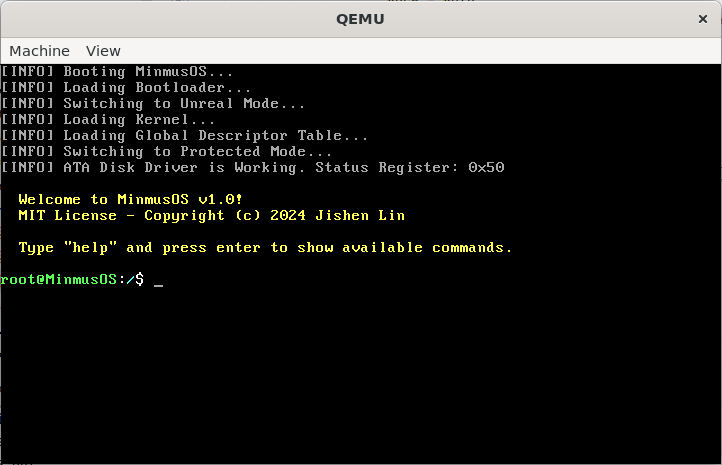
\includegraphics[width=0.8\textwidth]{figures/VGATextModePresentation.png}
    \caption{VGA文本模式演示}
    \label{fig:VGATextModePresentation}
\end{figure}

\subsection{内存管理(Memory Management)}

在MinmusOS中,内存管理由两个核心组件处理:内存分配器(Memory Allocator)和分页管理器(Paging Manager)。kernel/src/memory/allocator.rs定义了一个名为Allocator的内存分配器,它实现了Rust标准库的GlobalAlloc特质,提供了基本的内存分配和释放接口。kernel/src/memory/paging.rs包含分页管理逻辑,定义了PageDirectory和PageTable结构,用于处理虚拟地址到物理地址的映射。这包括设置页表、启用分页机制,并提供标识映射的功能,即将一系列预定义的虚拟地址直接映射到相同的物理地址。这样的内存管理设计旨在支持操作系统的基础内存操作需求,为更复杂的内存管理特性和优化提供基础。

\subsubsection{内存分配器(Memory Allocator)}

MinmusOS 的内存分配器设计相对简单,使用了单链表结构管理内存块。这种设计虽然易于实现和理解,但在复杂的场景下,可能会因为频繁的链表操作而导致性能瓶颈。因此,在未来版本中,可能需要考虑引入更高级的内存管理机制,如伙伴分配器或堆碎片整理策略,以提升内存分配的效率和鲁棒性。

\paragraph{\texttt{Block}数据结构}

Block 结构体(\cref{lst:BlockDataStructure})表示内存分配器中的一个内存块,包含两个字段:size 表示内存块的大小,next 是一个 \texttt{Option<NonNull<Block>>} 类型的字段,指向下一个内存块。自动派生的 Copy 和 Clone 特质使得 Block 结构体可以按值进行复制,Debug 特质允许对其进行调试输出。

\begin{listing}[htbp]
    \begin{minted}{rust}
#[derive(Copy, Clone, Debug)]
struct Block {
    size: usize,
    next: Option<NonNull<Block>>,
}
    \end{minted}
    \caption{\texttt{Block}数据结构}\label{lst:BlockDataStructure}
\end{listing}

\paragraph{\texttt{Allocator}数据结构}

Allocator 结构体(\cref{lst:AllocatorDataStructure})包含一个 \texttt{AtomicPtr<Block>} 类型的头指针 head,它指向一个内存块链表的起始位置。链表中的每个节点表示一个可用的内存块,其大小由 size 字段表示,next 字段指向下一个内存块。通过使用原子指针,Allocator 能够在多线程环境中安全地更新链表。

\begin{listing}[htbp]
    \begin{minted}{rust}
pub struct Allocator {
    head: AtomicPtr<Block>,
}
    \end{minted}
    \caption{\texttt{Allocator}数据结构}\label{lst:AllocatorDataStructure}
\end{listing}

init 方法(\cref{lst:AllocatorImplementation})用于初始化内存分配器的堆空间。该方法接受堆的起始地址和大小,并将堆视为一个大的空闲内存块。这个初始内存块被存储在 head 指针中,准备好供后续的分配操作使用。

\begin{listing}[htbp]
    \begin{minted}{rust}
impl Allocator {
    pub const fn new() -> Self {
        Allocator {
            head: AtomicPtr::new(ptr::null_mut())
        }
    }

    #[allow(dead_code)]
    pub unsafe fn init(&self, heap_start: usize, heap_size: usize) {
        let block = Block {
            size: heap_size,
            next: None,
        };
        let block_ptr: *mut Block = heap_start as *mut Block;
        ptr::write(block_ptr, block);
        self.head.store(block_ptr, Ordering::SeqCst);
    }
}
    \end{minted}
    \caption{\texttt{Allocator}数据结构实现}\label{lst:AllocatorImplementation}
\end{listing}

\subsubsection{全局分配器接口(GlobalAlloc Trait)}

\cref{lst:GlobalAllocAllocMethod}实现了 GlobalAlloc 特质中的 alloc 方法。该方法接受一个 Layout 参数,表示所需内存的大小和对齐要求。分配器会遍历内存块链表,找到第一个满足要求的内存块并将其分配出去。如果找到合适的块,它将更新链表头指针,指向下一个空闲块。

\begin{listing}[htbp]
    \begin{minted}{rust}
unsafe fn alloc(&self, layout: Layout) -> *mut u8 {
    let mut current: *mut Block = self.head.load(Ordering::SeqCst);
    let alloc_size: usize = layout.size().max(layout.align());
    while !current.is_null() {
        let current_block: &mut Block = &mut *current;
        if current_block.size >= alloc_size {
            self.head.store(current_block.next.map_or(ptr::null_mut(), |b| b.as_ptr()), Ordering::SeqCst);
            return current as *mut u8;
        }
        current = current_block.next.map_or(ptr::null_mut(), |b| b.as_ptr());
    }
    ptr::null_mut()
}
    \end{minted}
    \caption{alloc内存分配接口}\label{lst:GlobalAllocAllocMethod}
\end{listing}

\cref{lst:GlobalAllocDeallocMethod}实现了 GlobalAlloc 特质中的 dealloc 方法,用于释放已分配的内存。dealloc 方法会将释放的内存块重新插入到链表的头部,从而使其能够被未来的内存分配请求重用。

\begin{listing}[htbp]
    \begin{minted}{rust}
unsafe fn dealloc(&self, ptr: *mut u8, layout: Layout) {
    let mut new_block = Block {
        size: layout.size(),
        next: None,
    };
    new_block.next = NonNull::new(self.head.load(Ordering::SeqCst));
    let new_block_ptr: *mut Block = ptr as *mut Block;
    ptr::write(new_block_ptr, new_block);
    self.head.store(new_block_ptr, Ordering::SeqCst);
}
    \end{minted}
    \caption{dealloc内存释放接口}\label{lst:GlobalAllocDeallocMethod}
\end{listing}

这个内存分配器的实现为操作系统的基础内存管理提供了核心支持,允许操作系统在不同的场景中动态分配和释放内存资源,从而更好地支持应用程序的执行和资源管理。

\subsubsection{分页管理器(Paging Manager)}

分页管理器(Paging Manager)负责操作系统中的分页内存管理机制,通过维护分页目录(Page Directory)和页表(Page Table)来管理虚拟内存与物理内存的映射关系。分页管理器的核心任务包括创建和初始化分页结构,设置页表项,并启用分页模式,使系统能够在启用分页后正确映射和管理内存。

\paragraph{全局分页变量(Global Paging Variables)}

\cref{lst:GlobalPagingVariables}定义了操作系统分页管理中使用的全局分页变量,包括分页目录(Page Directory)和页表(Page Table)。这些变量在整个系统中是全局共享的,确保分页机制能够在各个模块中一致地运作。为了适应分页内存管理的需求,这些数据结构被静态定义,并且通过特定的内存对齐方式进行存储,以确保其高效且正确的访问。

全局变量 PAGING 定义了一个全局的分页目录,用于存储虚拟内存与物理内存的映射关系。分页目录包含1024个条目,每个条目对应一个页表指针。全局变量 TABLES 是一个包含16个页表的数组,这些页表用于进一步细化内存映射,每个页表也包含1024个条目,指向物理内存中的实际页。初始状态下,这些页表被定义为 NULL\_TABLE,即一个默认的空页表。

NULL\_TABLE 作为一个全局常量,被初始化为全零的页表,用于未被分配或尚未使用的页表项。这个设计确保了系统在初始状态下的安全性与稳定性,防止未初始化的页表带来的潜在问题。通过这些全局变量,操作系统能够高效地管理内存映射关系,为不同进程提供隔离和保护。

\begin{listing}[htbp]
    \begin{minted}{rust}
pub static mut PAGING: PageDirectory = PageDirectory { entries: [0x00000002; 1024] };
pub static mut TABLES: [PageTable; 16] = [NULL_TABLE; 16];
pub static NULL_TABLE: PageTable = PageTable { entries: [0; 1024] };
    \end{minted}
    \caption{全局分页变量}\label{lst:GlobalPagingVariables}
\end{listing}

\paragraph{分页目录(Page Directory)}

PageDirectory 数据结构(\cref{lst:PageDirectoryDataStructure})使用了一个长度为 1024 的 entries 数组,每个数组项为 32 位无符号整数类型(u32),用来存储页表的物理地址和控制标志。数组中的每个条目对应着 4MB 的虚拟内存范围,其内容是页表的起始地址加上分页控制位。这种设计允许操作系统通过访问 entries 数组的不同索引来管理不同的内存段。

PageDirectory 提供了几个关键的方法来操作分页目录:

\begin{enumerate}
    \item \textbf{set\_table 方法}:该方法用于将一个页表的地址设置到分页目录中的指定索引位置。具体实现上,它接受一个页表指针,将其转换为对应的物理地址,并将该地址与必要的控制位(例如存在位和读写位)进行按位或运算,最终存储在 entries 数组的指定位置。这确保了该页表在分页系统中被正确识别和使用。
    \item \textbf{enable 方法}:该方法用于启用分页模式。它首先将分页目录的地址加载到控制寄存器 CR3 中,然后通过修改 CR0 寄存器的相应标志位来启用分页功能。这个操作是分页机制中至关重要的一步,允许操作系统从此时开始使用分页来管理内存。
    \item \textbf{identity 方法}:该方法用于进行内存的身份映射(identity mapping),将特定的物理地址范围直接映射到相同的虚拟地址范围。在实现上,它遍历 TABLES 数组的前八个页表,将每个页表初始化为对应的物理地址区间,并将这些页表加载到分页目录的前八个条目中。这种映射方式通常用于内核空间的地址映射,确保内核在启用分页后能够继续正常访问内存。
\end{enumerate}

\begin{listing}[htbp]
    \begin{minted}{rust}
        #[repr(align(4096))]
pub struct PageDirectory {
    pub entries: [u32; 1024],
}

impl PageDirectory {
    pub fn set_table(&mut self, index: usize, table: &PageTable) {
        self.entries[index] = (table as *const PageTable) as u32 | 0b011;
    }

    pub fn enable(&self) {
        unsafe {
            let address: u32 = (self as *const PageDirectory) as u32;
            core::arch::asm!(
            "mov cr3, eax",
            "mov eax, cr0",
            "or eax, 0x80000001",
            "mov cr0, eax",
            in("eax") address,
            );
        }
    }

    pub fn identity(&mut self) {
        unsafe {
            for i in 0..8 {
                TABLES[i].set((0x00400000 * i) as u32);
                PAGING.set_table(i, &TABLES[i]);
            }
        }
    }
}
    \end{minted}
    \caption{\texttt{PageDirectory}数据结构}\label{lst:PageDirectoryDataStructure}
\end{listing}

\paragraph{页表(Page Table)}

PageTable 数据结构由一个长度为 1024 的 entries 数组构成,每个数组项为 32 位无符号整数类型(u32),用于存储指向具体物理内存页的地址和相关的控制位。该数据结构被定义为带有 4096 字节对齐的结构体,确保页表在内存中的对齐要求与分页机制保持一致。这种对齐方式是分页系统中至关重要的一部分,有助于提高内存访问的效率和准确性。

在 PageTable 结构体(\cref{lst:PageTableDataStructure})中,每个 entries 数组元素对应一个 4KB 的内存页,因此整个 PageTable 能够管理 4MB 的虚拟内存范围。每个数组项存储的内容包括物理页的起始地址以及一些控制位,这些控制位用于指定页面是否存在、可读写、用户权限等。

PageTable 提供了 set 方法。set 方法用于初始化页表中的所有条目,将它们映射到一个从指定起始地址开始的物理内存范围。方法接受一个 from 参数,表示物理地址的起始点。方法通过循环遍历 entries 数组,将每个条目设置为一个物理页的地址和相关的控制位。具体地,物理地址的计算是通过将数组索引乘以页面大小(4KB)并加上 from 参数来实现的。控制位则通过按位或运算加入到地址中,通常包括页面的存在位和读写权限位。这种方式允许操作系统将连续的一段虚拟地址映射到连续的物理地址,提供了对内存的有效管理。

\begin{listing}[htbp]
    \begin{minted}{rust}
#[derive(Copy, Clone, Debug)]
#[repr(align(4096))]
pub struct PageTable {
    pub entries: [u32; 1024],
}

impl PageTable {
    pub fn set(&mut self, from: u32) {
        for i in 0..1024 {
            self.entries[i] = (((i * 0x1000) + from as usize) | 0b011) as u32;
        }
    }
}
    \end{minted}
    \caption{\texttt{PageTable}数据结构}\label{lst:PageTableDataStructure}
\end{listing}

\subsubsection{分页目录(Page Directory)与页表(Page Table)}

\cref{fig:PageDirectoryAndPageTable}展示了分页目录与页表的结构与联系。

分页目录是分页机制的第一层结构,用于管理整个虚拟内存空间的映射。一个分页目录包含1024个条目,每个条目指向一个页表。分页目录本身的每个条目管理着一个大的虚拟地址块,通常是4MB的虚拟内存。因此,分页目录的主要作用是将虚拟地址空间划分成更小的段,并通过页表进一步细化这些段的地址映射。

页表是分页机制的第二层结构,用于细化虚拟地址到物理地址的映射。每个页表也包含1024个条目,每个条目对应一个4KB的物理内存页。因此,页表的作用是将从分页目录获得的虚拟地址范围进一步分解,精确映射到物理内存的具体页面。

\begin{figure}[htbp]
    \centering
    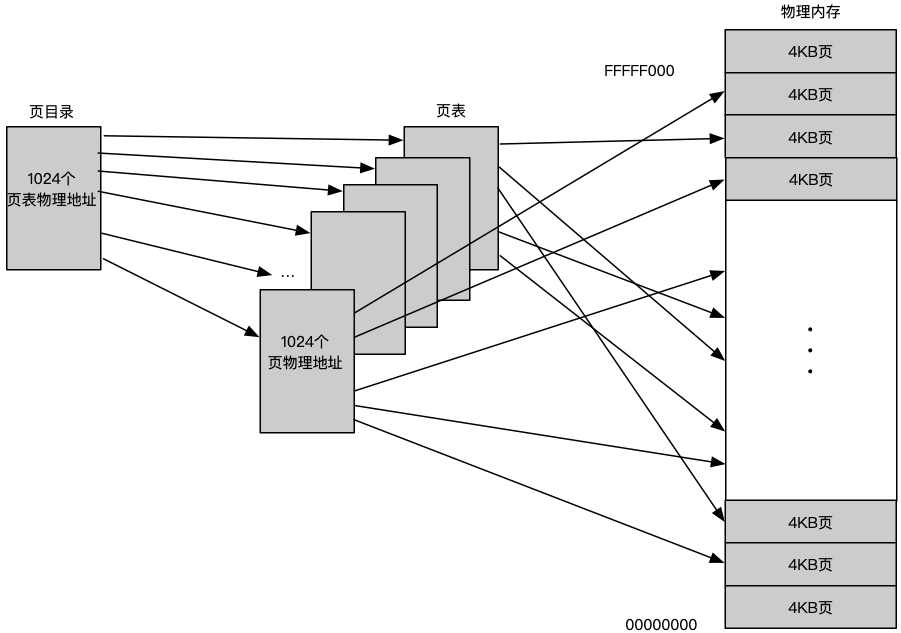
\includegraphics[width=0.8\textwidth]{figures/PageDirectoryAndPageTable.png}
    \caption{分页目录与页表}
    \label{fig:PageDirectoryAndPageTable}
\end{figure}

分页目录的主要功能是通过其条目指向不同的页表,从而管理大块虚拟地址空间。它起到了一个索引的作用,将虚拟地址的高位部分映射到对应的页表。页表的功能是将分页目录指向的虚拟地址块进一步细化,映射到具体的物理内存页。它完成了从虚拟地址到物理地址的最终转换。

分页管理器通过组合分页目录和页表,提供了一种灵活的内存管理机制,使得操作系统能够有效地管理和保护内存资源,支持多任务和内存隔离的实现。

\subsection{文件系统(File System)}

\subsubsection{FAT16文件系统}

FAT16(File Allocation Table 16-bit,16位文件分配表)是微软最早开发的文件系统之一,最早在MS-DOS操作系统中引入。FAT16的设计目的是为了在早期的磁盘驱动器上高效地管理文件和目录。以下是FAT16文件系统的详细介绍:

\begin{enumerate}
    \item \textbf{文件分配表(FAT)}:FAT是文件系统的核心部分,用于记录每个文件在磁盘上的存储位置。FAT表本质上是一个链表,每个文件由多个簇(Cluster)组成,而每个簇对应于FAT表中的一个条目。FAT表记录了每个簇的下一个簇的位置,文件的最后一个簇标记为0xFFFF,表示文件结束。
          \begin{enumerate}
              \item \textbf{16位条目}:FAT16使用16位条目来表示每个簇的索引,因此它最多可以管理 $2^16 = 65536$ 个簇。
              \item \textbf{簇链}:文件在磁盘上的簇可能不是连续存储的,FAT表将这些分散的簇链在一起,形成文件的完整数据。
          \end{enumerate}
    \item \textbf{簇(Cluster)}:簇是FAT文件系统中磁盘的基本分配单位。簇由多个扇区(通常为512字节)组成,文件在磁盘上的存储是以簇为单位进行分配的。簇的大小决定了文件系统的最大容量和性能。
          \begin{enumerate}
              \item \textbf{簇大小}:通常簇大小为4KB、8KB或更大,具体取决于磁盘的大小。较大的簇有助于减少FAT表的大小,但也可能导致磁盘空间浪费(特别是存储小文件时)。
          \end{enumerate}
    \item \textbf{文件和目录}:在FAT16文件系统中,文件和目录的信息存储在根目录和子目录中。每个文件和目录的元数据保存在一个32字节的目录项中。
          \begin{enumerate}
              \item \textbf{文件名}:FAT16使用8.3格式(8个字符的文件名加上3个字符的扩展名)来表示文件名。
              \item \textbf{目录结构}:目录也是一种文件,它包含子目录和文件的列表。根目录有固定的大小,不能动态扩展。
              \item \textbf{元数据}:每个目录项包含文件或目录的名称、文件大小、起始簇号、创建时间、修改时间、属性(如只读、隐藏、系统文件等)等信息。
          \end{enumerate}
    \item \textbf{扇区(Sector)和磁盘布局}:磁盘在FAT16文件系统中按照一定的布局分为多个区域,每个区域有特定的功能:
          \begin{enumerate}
              \item \textbf{引导扇区(Boot Sector)}:磁盘的第一个扇区,包含引导程序和文件系统的基本信息,如每簇的扇区数、FAT表的起始位置、根目录的起始位置等。
              \item \textbf{FAT表区域}:存放FAT表的数据,通常有两份FAT表用于冗余备份。
              \item \textbf{根目录区域}:存放根目录的目录项,FAT16的根目录区大小固定,通常位于FAT表之后。
              \item \textbf{数据区}:存放实际文件和目录数据,由簇构成。
          \end{enumerate}
    \item \textbf{文件操作}:在FAT16中,文件的操作包括创建、删除、读取和写入文件等。这些操作都是通过更新FAT表和目录项来实现的。
          \begin{enumerate}
              \item \textbf{创建文件}:在根目录或子目录中创建一个新的目录项,为文件分配簇,并在FAT表中记录簇链。
              \item \textbf{删除文件}:标记目录项为删除,并释放FAT表中对应的簇。
              \item \textbf{读取文件}:根据目录项中的起始簇号,遍历FAT表获取文件的所有簇,并读取这些簇的数据。
              \item \textbf{写入文件}:找到文件的空闲簇,更新FAT表和目录项,将数据写入相应的簇。
          \end{enumerate}
    \item \textbf{限制和特点}:由于使用16位的簇索引,FAT16的最大卷大小为2GB(如果使用32KB的簇),且文件名必须遵循8.3格式,这对文件命名有一定的限制。此外FAT16没有内建的文件权限管理功能,不支持复杂的安全策略。
\end{enumerate}

\subsubsection{FAT16全局常量定义}

\cref{lst:FAT16GlobalConstantDefinitions}在 FAT16 文件系统实现中分别定义了以下内容:

\begin{enumerate}
    \item \texttt{ENTRY\_COUNT}:定义了根目录中最多可以容纳的目录项数量为 512,用于限制根目录的文件和子目录数量。
    \item \texttt{FAT\_START}:指定了文件分配表(FAT)在磁盘上的起始位置(逻辑块地址 LBA),其值为 36864,用于定位 FAT 表在磁盘上的位置。
    \item \texttt{FAT\_SIZE}:定义了 FAT 表的大小为 256,表示 FAT 表中可以存储的簇链条目数量,用于跟踪文件在磁盘上的簇链。
\end{enumerate}

\begin{listing}[htbp]
    \begin{minted}{rust}
const ENTRY_COUNT: usize = 512;
const FAT_START: u16 = 36864;
const FAT_SIZE: usize = 256;
    \end{minted}
    \caption{FAT16全局常量定义}\label{lst:FAT16GlobalConstantDefinitions}
\end{listing}

\subsubsection{Header数据结构}

Header 结构体(\cref{lst:HeaderDataStructure})表示 FAT16 文件系统的引导扇区信息,用于存储文件系统的元数据,包括引导加载器代码、文件系统参数(如扇区大小、簇大小、FAT 表数量等)、卷标信息和保留区域。这个结构体在加载 FAT16 文件系统时至关重要,因为它提供了文件系统布局的基本信息,帮助操作系统正确解析和操作磁盘上的数据。

\begin{listing}[htbp]
    \begin{minted}{rust}
#[derive(Copy, Clone, Debug)]
#[repr(C, packed)]
pub struct Header {
    boot_jump_instructions: [u8; 3], // 引导跳转指令,用于启动时跳转到引导程序
    oem_identifier: [u8; 8],         // OEM 标识符,标识文件系统创建的操作系统或工具
    bytes_per_sector: u16,           // 每扇区字节数,通常为 512 字节
    sectors_per_cluster: u8,         // 每簇包含的扇区数,决定了簇的大小
    reserved_sectors: u16,           // 保留扇区数,通常包括引导扇区和其他保留数据
    fat_count: u8,                   // FAT 表的数量,通常为 2,用于冗余备份
    dir_entries_count: u16,          // 根目录的目录项数量,表示根目录最多可以容纳的文件和目录数量
    total_sectors: u16,              // 总扇区数,如果为 0,则使用 large_sector_count 字段
    media_descriptor_type: u8,       // 媒体描述符类型,标识存储设备的类型
    sectors_per_fat: u16,            // 每个 FAT 表占用的扇区数
    sectors_per_track: u16,          // 每个磁道的扇区数,用于 CHS(柱面-磁头-扇区)寻址模式
    heads: u16,                      // 磁头数,用于 CHS 寻址模式
    hidden_sectors: u32,             // 隐藏扇区数,表示从磁盘起始到分区起始之间的扇区数
    large_sector_count: u32,         // 总扇区数(如果 total_sectors 为 0),用于支持大于 32MB 的卷
    drive_number: u8,                // 驱动器号,通常为 0x80 表示硬盘
    reserved: u8,                    // 保留字段,通常为 0,未使用
    signature: u8,                   // 扩展引导签名,用于验证引导扇区是否有效
    volume_id: u32,                  // 卷序列号,用于唯一标识卷
    volume_label: [u8; 11],          // 卷标,用于显示卷的名称
    system_id: [u8; 8],              // 文件系统类型标识符,如 "FAT16   "
    zero: [u8; 460],                 // 填充字段,通常为 0,用于对齐和保留空间
}
    \end{minted}
    \caption{\texttt{Header}数据结构}\label{lst:HeaderDataStructure}
\end{listing}

NULL\_HEADER 是一个用于初始化 Header 结构体的静态变量,其作用是提供一个默认的、空的 FAT16 文件系统头部信息。当创建或初始化一个 Header 变量时,如果尚未从磁盘加载实际的文件系统信息,可以使用 NULL\_HEADER 作为占位符。它确保在没有加载有效数据之前,Header 结构体中的字段都被安全地设置为默认值(通常是零或空值),防止意外访问未初始化的数据。

\subsubsection{Entry数据结构}

Entry 结构体(\cref{lst:EntryDataStructure})表示 FAT16 文件系统中的目录项,用于存储文件或目录的元数据。每个目录项包含文件的名称、属性、创建和修改时间、文件的起始簇号以及文件大小等信息。这个结构体是 FAT16 文件系统管理文件和目录的基础单元,它通过这些元数据来描述文件在磁盘上的位置和相关属性,从而使操作系统能够正确地访问和管理文件。

\begin{listing}[htbp]
    \begin{minted}{rust}
#[derive(Copy, Clone, Debug)]
#[repr(C, packed)]
pub struct Entry {
    pub name: [u8; 11],      // 文件名,采用 8.3 格式(8 个字符的文件名 + 3 个字符的扩展名)
    attributes: u8,          // 文件属性,如只读、隐藏、系统文件等
    reserved: u8,            // 保留字段,未使用
    created_time_tenths: u8, // 文件创建时间的十分之一秒,用于提高时间精度
    created_time: u16,       // 文件创建时间(小时、分钟、秒)
    created_date: u16,       // 文件创建日期(年、月、日)
    accessed_date: u16,      // 最近访问日期
    first_cluster_high: u16, // 文件的起始簇号高 16 位(仅用于 FAT32,FAT16 中未使用)
    modified_time: u16,      // 最近修改时间(小时、分钟、秒)
    modified_date: u16,      // 最近修改日期(年、月、日)
    first_cluster_low: u16,  // 文件的起始簇号低 16 位,指向文件内容在数据区的起始位置
    size: u32,               // 文件大小,以字节为单位
}
    \end{minted}
    \caption{\texttt{Entry}数据结构}\label{lst:EntryDataStructure}
\end{listing}

NULL\_ENTRY 是一个用于初始化 Entry 结构体的静态变量,其作用是提供一个默认的、空的目录项。当创建或初始化一个 Entry 变量时,如果尚未加载实际的文件或目录信息,可以使用 NULL\_ENTRY 作为占位符。它的存在确保在遍历或操作目录项时,如果遇到无效或空的目录项,能够安全地返回 NULL\_ENTRY,从而避免处理无效数据,保持程序的稳定性和安全性。

\subsubsection{FatDriver数据结构}

FatDriver 结构体(\cref{lst:FatDriverDataStructure})是 FAT16 文件系统驱动程序的核心数据结构,设计用于管理和操作文件系统。它包含四个关键部分:header 存储 FAT16 文件系统的引导扇区信息,entries 存储根目录中的所有目录项,table 存储文件分配表(FAT),buffer 用于临时存储从磁盘读取的文件数据。通过这种设计,FatDriver 能够全面管理 FAT16 文件系统的基本操作,包括文件和目录的读取、写入以及簇链的管理。

\begin{listing}[htbp]
    \begin{minted}{rust}
#[derive(Copy, Clone, Debug)]
pub struct FatDriver {
    pub header: Header,
    pub entries: [Entry; ENTRY_COUNT],
    pub table: [u16; FAT_SIZE],
    pub buffer: [u8; 2048],
}
    \end{minted}
    \caption{\texttt{FatDriver}数据结构}\label{lst:FatDriverDataStructure}
\end{listing}

FAT 是一个全局静态变量(\cref{lst:FATGlobalStaticVariable}),使用 Mutex 保护 FatDriver 实例,以确保线程安全。它在程序启动时被初始化,将 header、entries 和 table 等结构体字段设置为默认的空值或零值,防止未初始化的访问。在实际操作过程中,FAT 作为整个 FAT16 文件系统的入口点,负责管理和调度文件系统的各种操作。

\begin{listing}[htbp]
    \begin{minted}{rust}
pub static mut FAT: Mutex<FatDriver> = Mutex::new(FatDriver {
    header: NULL_HEADER,
    entries: [NULL_ENTRY; ENTRY_COUNT],
    table: [0; FAT_SIZE],
    buffer: [0; 2048],
});
    \end{minted}
    \caption{FAT全局静态变量}\label{lst:FATGlobalStaticVariable}
\end{listing}

\subsubsection{FAT16文件操作}

\paragraph{加载文件系统头部信息}

load\_header 方法(\cref{lst:LoadHeaderMethod})用于从磁盘的指定位置(由 FAT\_START 和 reserved\_sectors 决定)加载 FAT16 文件系统的头部信息(Header 结构体)到 FatDriver 的 header 字段中。这个操作是文件系统初始化的第一步,获取文件系统的基本参数如每扇区字节数、每簇扇区数等,为后续文件操作提供必要的元数据。

\begin{listing}[htbp]
    \begin{minted}{rust}
pub fn load_header(&mut self) {
    let target: *mut Header = &mut self.header as *mut Header;
    let lba: u64 = FAT_START as u64;
    let sectors: u16 = 1;
    unsafe { DISK.read(target, lba, sectors); }
}
    \end{minted}
    \caption{load\_header 方法}\label{lst:LoadHeaderMethod}
\end{listing}

\paragraph{加载根目录的目录项}

load\_entries 方法(\cref{lst:LoadEntriesMethod})从磁盘中加载根目录的所有目录项到 entries 数组中。通过计算目录项的起始逻辑块地址(LBA)和所需的扇区数,该方法将所有目录项数据从磁盘读取到内存中,以便后续对文件和目录的操作。根目录的目录项包含文件和子目录的元数据。

\begin{listing}[htbp]
    \begin{minted}{rust}
pub fn load_entries(&mut self) {
    let target: *mut Entry = &mut self.entries as *mut Entry;
    let entry_size: u16 = size_of::<Entry>() as u16;
    let lba: u64 = FAT_START as u64 + (self.header.reserved_sectors + self.header.sectors_per_fat * self.header.fat_count as u16) as u64;
    let size: u16 = entry_size * self.header.dir_entries_count;
    let sectors: u16 = size / self.header.bytes_per_sector;
    unsafe { DISK.read(target, lba, sectors); }
}
    \end{minted}
    \caption{load\_entries 方法}\label{lst:LoadEntriesMethod}
\end{listing}

\paragraph{列出根目录中的文件和目录}

list\_entries 方法(\cref{lst:ListEntriesMethod})遍历 entries 数组,并列出其中所有有效的目录项(文件或目录),打印出每个文件的名称和大小。这一方法用于展示根目录中的内容,帮助用户或系统查看文件系统中存在哪些文件和目录。

\begin{listing}[htbp]
    \begin{minted}{rust}
pub fn list_entries(&self) {
    lib::println!("Filename     Size");
    for i in 0..ENTRY_COUNT {
        if self.entries[i].name[0] != 0 {
            for c in self.entries[i].name { lib::print!("{}", c as char); }
            let size = self.entries[i].size;
            lib::println!("  {} bytes", size);
        }
    }
}
    \end{minted}
    \caption{list\_entries 方法}\label{lst:ListEntriesMethod}
\end{listing}

\paragraph{加载文件分配表(FAT 表)}

load\_table 方法(\cref{lst:LoadTableMethod})从磁盘加载文件分配表(FAT)到 table 数组中。FAT 表记录了文件在磁盘上的簇链信息,表示文件的各个部分(簇)在磁盘中的物理位置。这个方法是文件读取和写入操作的前提,通过 FAT 表可以找到文件的所有数据块。

\begin{listing}[htbp]
    \begin{minted}{rust}
pub fn load_table(&mut self) {
    let target: *mut u16 = &mut self.table as *mut u16;
    let lba: u64 = FAT_START as u64 + self.header.reserved_sectors as u64;
    let sectors: u16 = 1;
    unsafe { DISK.read(target, lba, sectors); }
}
    \end{minted}
    \caption{load\_table 方法}\label{lst:LoadTableMethod}
\end{listing}

\paragraph{将文件内容读取到缓冲区}

read\_file\_to\_buffer 方法(\cref{lst:ReadFileToBufferMethod})用于将指定文件的内容从磁盘读取到 buffer 缓冲区中。它通过计算文件数据的起始 LBA,并使用 FAT 表找到文件的所有簇链,读取文件的内容到内存中的缓冲区中。这个方法适用于读取小文件或进行临时处理的场景。

\begin{listing}[htbp]
    \begin{minted}{rust}
pub fn read_file_to_buffer(&self, entry: &Entry) {
    let target: *mut u8 = self.buffer.as_ptr() as *mut u8;
    let data_lba: u64 = FAT_START as u64 + (self.header.reserved_sectors + self.header.sectors_per_fat * self.header.fat_count as u16 + 32) as u64;
    let lba: u64 = data_lba + ((entry.first_cluster_low - 2) * self.header.sectors_per_cluster as u16) as u64;
    let sectors: u16 = self.header.sectors_per_cluster as u16;
    unsafe { DISK.read(target, lba, sectors); }
}
    \end{minted}
    \caption{read\_file\_to\_buffer 方法}\label{lst:ReadFileToBufferMethod}
\end{listing}

\paragraph{将文件内容读取到指定目标内存}

read\_file\_to\_target 方法(\cref{lst:ReadFileToTargetMethod})用于将文件的内容从磁盘读取到指定的目标内存位置。该方法通过遍历 FAT 表,逐簇读取文件内容,并将其写入目标内存地址,直到文件的最后一个簇。这种操作适用于需要将文件内容直接加载到指定内存区域的场景,如加载可执行文件。

\paragraph{在目录中搜索文件}

search\_file 方法(\cref{lst:SearchFileMethod})在 entries 数组中搜索指定名称的文件或目录,并返回对应的目录项(Entry 结构体)。它逐个比较目录项中的文件名与目标名称,忽略大小写,并返回找到的文件或目录的元数据。如果未找到,返回 NULL\_ENTRY 作为占位符。这个方法用于查找文件系统中的具体文件或目录。

\subsubsection{示例文本文件}

MinmusOS提供了五个示例文本文件,加载到了根目录中:

\begin{enumerate}
    \item \textbf{cargo}:Cargo包管理器介绍。(\cref{fig:CargoFilePresentation})
    \item \textbf{license}:MinmusOS项目MIT许可证文件。(\cref{fig:LicenseFilePresentation})
    \item \textbf{minmusos}:MinmusOS欢迎文件与联系方式。(\cref{fig:MinmusOSFilePresentation})
    \item \textbf{rust}:Rust语言介绍。(\cref{fig:RustFilePresentation})
    \item \textbf{thanks}:致谢。(\cref{fig:ThanksFilePresentation})
\end{enumerate}

可以在命令行解释器(Shell)中通过cat命令查看这些文件。

\begin{listing}[htbp]
    \begin{minted}{rust}
pub fn read_file_to_target(&self, entry: &Entry, target: *mut u32) {
    let mut next_cluster: u16 = entry.first_cluster_low;
    let mut current_target: *mut u32 = target;
    loop {
        let data_lba: u64 = FAT_START as u64 + (self.header.reserved_sectors + self.header.sectors_per_fat * self.header.fat_count as u16 + 32) as u64;
        let lba: u64 = data_lba + ((next_cluster - 2) * self.header.sectors_per_cluster as u16) as u64;
        let sectors: u16 = self.header.sectors_per_cluster as u16;
        unsafe { DISK.read(current_target, lba, sectors); }
        next_cluster = self.table[next_cluster as usize];
        unsafe {
            let cluster_size: u16 = self.header.sectors_per_cluster as u16 * self.header.bytes_per_sector;
            current_target = current_target.byte_add(cluster_size as usize);
        }
        if next_cluster == 0xFFFF { break; }
    }
}
    \end{minted}
    \caption{read\_file\_to\_target 方法}\label{lst:ReadFileToTargetMethod}
\end{listing}

\begin{listing}[htbp]
    \begin{minted}{rust}
pub fn search_file(&self, name: &[char]) -> &Entry {
    for entry in self.entries.iter() {
        let mut found: bool = true;
        let mut i: usize = 0;
        for n in name {
            let mut c: char = n.clone();
            if c.is_ascii_lowercase() { c = c.to_ascii_uppercase(); }
            if (c != entry.name[i] as char) && (name[i] != '\0') { found = false; }
            i += 1;
        }
        if found {
            return entry;
        }
    }
    &NULL_ENTRY
}
    \end{minted}
    \caption{search\_file 方法}\label{lst:SearchFileMethod}
\end{listing}

\begin{figure}[htbp]
    \centering
    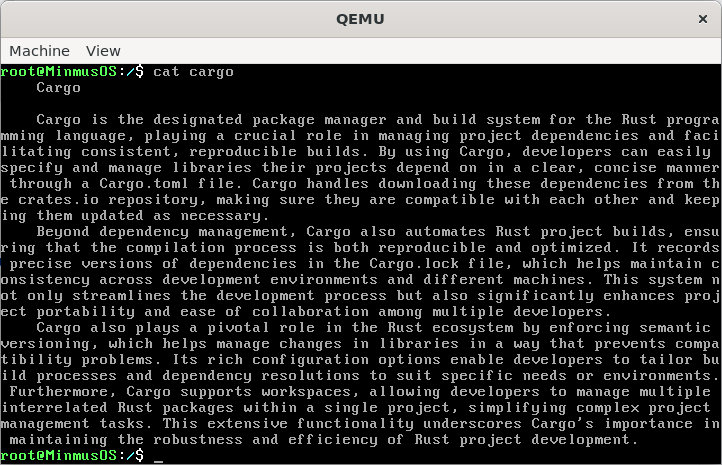
\includegraphics[width=0.8\textwidth]{figures/CargoFilePresentation.png}
    \caption{文本文件cargo演示}
    \label{fig:CargoFilePresentation}
\end{figure}

\begin{figure}[htbp]
    \centering
    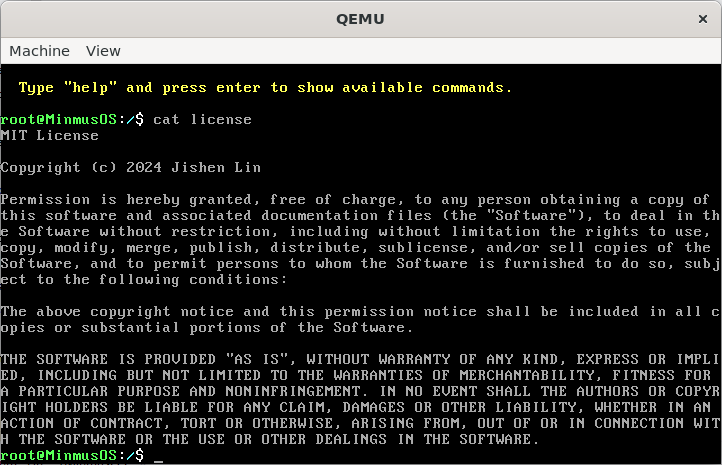
\includegraphics[width=0.8\textwidth]{figures/LicenseFilePresentation.png}
    \caption{文本文件license演示}
    \label{fig:LicenseFilePresentation}
\end{figure}

\begin{figure}[htbp]
    \centering
    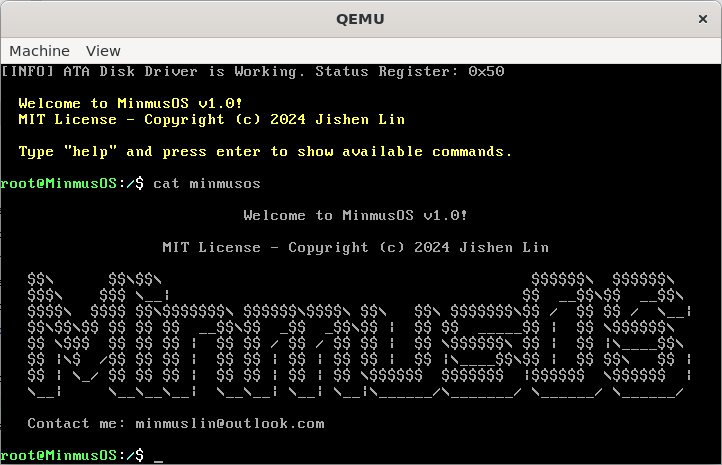
\includegraphics[width=0.8\textwidth]{figures/MinmusOSFilePresentation.png}
    \caption{文本文件minmusos演示}
    \label{fig:MinmusOSFilePresentation}
\end{figure}

\begin{figure}[htbp]
    \centering
    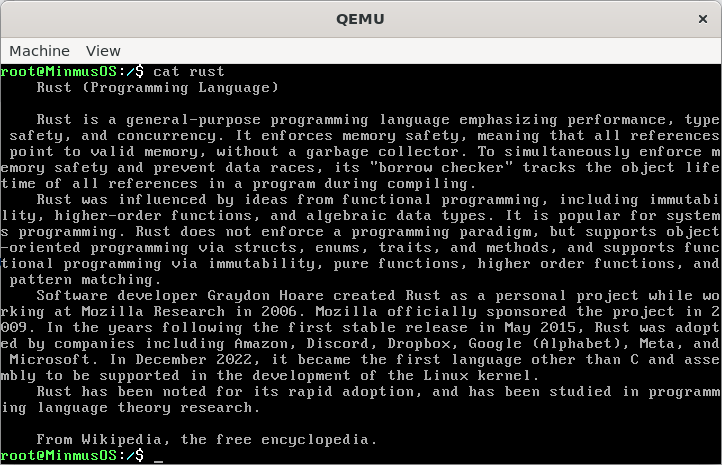
\includegraphics[width=0.8\textwidth]{figures/RustFilePresentation.png}
    \caption{文本文件rust演示}
    \label{fig:RustFilePresentation}
\end{figure}

\begin{figure}[htbp]
    \centering
    
\includegraphics[width=0.8\textwidth]{figures/ThanksFilePresentation.png}
    \caption{文本文件thanks演示}
    \label{fig:ThanksFilePresentation}
\end{figure}

\subsection{定时器(Timer)}

在操作系统内核中,定时器(Timer)是一种核心组件,用于测量和控制时间的流逝,支持任务调度、超时管理、和性能监测等关键功能。它可以基于硬件也可以基于软件实现,确保操作系统能有效地管理和分配处理器时间,从而维持系统的高效运行和响应性。定时器的精确操作对于实现多任务处理、实时系统的需求和系统稳定性至关重要,使其成为任何现代操作系统不可或缺的组成部分。

\subsubsection{日期时间(Datetime)}

Time 数据结构(\cref{lst:TimeDataStructure})用于封装日期和时间信息,包括年、月、日、小时、分钟和秒。此结构体还包含用于记录自Unix纪元以来的秒数的时间戳(timestamp)和CPU时钟周期数(ticks),这使得它可以为操作系统提供精确的时间跟踪和性能监测功能。Time 结构体的设计允许系统在执行任务调度、时间管理和资源监控等操作时,能够高效且准确地处理时间相关数据。这种数据结构的实现,是操作系统能够提供稳定和可靠服务的基础之一。

\begin{listing}[htbp]
    \begin{minted}{rust}
#[derive(Copy, Clone, Debug)]
pub struct Time {
    year: u16,
    month: u8,
    day: u8,
    hour: u8,
    minute: u8,
    second: u8,
    timestamp: u64,
    ticks: u64,
}
    \end{minted}
    \caption{\texttt{Time}数据结构}\label{lst:TimeDataStructure}
\end{listing}

\cref{lst:GetCurrentDatetimeMethod}定义的 get\_current\_datetime() 函数是用于从硬件的实时时钟(RTC)\footnote{RTC(Real-Time Clock)即实时时钟,是计算机系统中的一种硬件设备,用于维持当前的日期和时间。即使在计算机断电或重启的情况下,它也能够继续运行,这是因为RTC通常由一个小电池供电,这使得它能在没有外部电源时持续工作。}中直接获取当前的日期和时间。该函数返回一个元组,包含年、月、日、小时、分钟和秒,格式为 \texttt{(u16, u8, u8, u8, u8, u8)}。这种方法通常用于操作系统级别的时间管理,如设置系统时钟或执行与时间相关的操作。

函数利用 x86 I/O 指令 out 和 in 来读取 RTC 的时间数据。例如,通过设置 RTC 寄存器地址并读取对应的数据,从而分别获取秒、分钟、小时、日、月、年的值。每个时间部分的数据都是通过一系列的内联汇编命令独立获取的。

读取的时间数据通常以二进制编码十进制(BCD)格式返回,其中每个字节的两个半字节分别表示十位和个位。函数 \texttt{bcd\_to\_binary(bcd: u8) -> u8} 负责将这些BCD编码的数据转换为普通的二进制整数值,转换方式是将低半字节的值加上高半字节值乘以10。

在处理完所有的时间数据后,由于读取的年份是从2000年开始的偏移量,函数会将这个偏移量加上2000来得到完整的年份。最后,函数将这些处理过的数据组装成一个元组返回。

由于直接进行硬件访问和使用内联汇编,这些操作被包裹在 unsafe 代码块中,以标识潜在的风险。

\begin{listing}[htbp]
    \begin{minted}{rust}
fn get_current_datetime() -> (u16, u8, u8, u8, u8, u8) {
    let mut second: u8;
    let mut minute: u8;
    let mut hour: u8;
    let mut day: u8;
    let mut month: u8;
    let mut year: u8;
    unsafe {
        asm!(
        "out 0x70, al",
        "in al, 0x71",
        in("al") 0x00u8,
        lateout("al") second,
        );
        asm!(
        "out 0x70, al",
        "in al, 0x71",
        in("al") 0x02u8,
        lateout("al") minute,
        );
        asm!(
        "out 0x70, al",
        "in al, 0x71",
        in("al") 0x04u8,
        lateout("al") hour,
        );
        asm!(
        "out 0x70, al",
        "in al, 0x71",
        in("al") 0x07u8,
        lateout("al") day,
        );
        asm!(
        "out 0x70, al",
        "in al, 0x71",
        in("al") 0x08u8,
        lateout("al") month,
        );
        asm!(
        "out 0x70, al",
        "in al, 0x71",
        in("al") 0x09u8,
        lateout("al") year,
        );
    }
    second = Self::bcd_to_binary(second);
    minute = Self::bcd_to_binary(minute);
    hour = Self::bcd_to_binary(hour);
    day = Self::bcd_to_binary(day);
    month = Self::bcd_to_binary(month);
    year = Self::bcd_to_binary(year);
    (2000 + year as u16, month, day, hour, minute, second)
}
    \end{minted}
    \caption{get\_current\_datetime方法}\label{lst:GetCurrentDatetimeMethod}
\end{listing}

\subsubsection{UNIX时间戳(UNIX Timestamp)}

UNIX时间戳(UNIX Timestamp),也称为POSIX时间或Epoch时间,是一种广泛使用的时间表示方法,其定义为自1970年1月1日00:00:00协调世界时(UTC)起至当前时刻的总秒数,不计入闰秒。UNIX时间戳为整型数字,便于计算机系统进行日期和时间的计算与比较。它是操作系统、数据库和各类应用程序中处理时间的一种基准格式,允许简便地进行时间的加减和转换。由于其简单和一致性,UNIX时间戳在全球范围内被广泛应用于多种编程环境和网络协议中。

\cref{lst:GetUnixTimestampMethod}实现了一个函数 get\_unix\_timestamp,该函数用于将给定的日期时间元组转换为自1970年1月1日00:00:00 UTC以来的总秒数,即UNIX时间戳。

\begin{listing}[htbp]
    \begin{minted}{rust}
fn get_unix_timestamp(datetime: (u16, u8, u8, u8, u8, u8)) -> u64 {
    let (year, month, day, hour, minute, second) = datetime;
    let mut days_since_epoch: u64 = 0;
    for y in 1970..year {
        days_since_epoch += if Self::is_leap_year(y) { 366 } else { 365 };
    }
    let month_days: [i32; 13] = if Self::is_leap_year(year) {
        [0, 31, 29, 31, 30, 31, 30, 31, 31, 30, 31, 30, 31]
    } else {
        [0, 31, 28, 31, 30, 31, 30, 31, 31, 30, 31, 30, 31]
    };
    for m in 1..month {
        days_since_epoch += month_days[m as usize] as u64;
    }
    days_since_epoch += day as u64 - 1;
    let hours_since_epoch: u64 = days_since_epoch * 24 + hour as u64;
    let minutes_since_epoch: u64 = hours_since_epoch * 60 + minute as u64;
    let seconds_since_epoch: u64 = minutes_since_epoch * 60 + second as u64;
    seconds_since_epoch
}
    \end{minted}
    \caption{get\_unix\_timestamp方法}\label{lst:GetUnixTimestampMethod}
\end{listing}

\subsubsection{CPU时钟周期计数(CPU Ticks)}

CPU时钟周期计数(CPU Ticks)是指在中央处理器(CPU)中进行操作的基本时间单位,每个时钟周期代表CPU完成其基本操作的能力的一个周期。这些时钟周期通过使用特定的硬件指令,如 x86 架构的 rdtsc(Read Time-Stamp Counter),直接从CPU的时间戳计数器中读取。CPU时钟周期数提供了一种测量代码执行时间和系统性能的直接方法,常用于性能优化、系统监测、和精确的时间测量。由于每个时钟周期的持续时间取决于CPU的时钟频率,所以它可以作为评估不同CPU和不同环境下程序性能的重要指标。

get\_cpu\_ticks() 函数(\cref{lst:GetCpuTicksMethod})用于获取 CPU 的时钟周期计数,即 CPU Ticks,这是衡量处理器执行时间的一个基本单位。函数使用 x86 架构的 rdtsc 指令来读取 CPU 的时间戳计数器。在执行 rdtsc 指令时,时钟周期的计数被分为高位和低位存储。eax 寄存器存储低32位,而 edx 寄存器存储高32位。通过位操作将高位和低位组合成一个 64 位的整数。具体操作是将高位(high)左移32位,然后与低位(low)进行位或操作(|),这样就能得到一个完整的 64 位的时钟周期计数。

由于 rdtsc 指令获取的是从 CPU 启动到当前的总时钟周期数,可以用来精确测量代码执行的时间,这是性能分析和优化中常用的一种方法。

\begin{listing}[htbp]
    \begin{minted}{rust}
fn get_cpu_ticks() -> u64 {
    let mut low: u32;
    let mut high: u32;
    unsafe {
        asm!(
        "rdtsc",
        out("eax") low,
        out("edx") high,
        options(nostack, nomem),
        );
    }
    ((high as u64) << 32) | (low as u64)
}
    \end{minted}
    \caption{get\_cpu\_ticks方法}\label{lst:GetCpuTicksMethod}
\end{listing}

\subsection{命令行解释器(Shell)}

命令行解释器(Shell)是一个用户界面,用于向操作系统提供用户指令。用户可以通过键入命令来与系统交互,这些命令然后由 Shell 解释并传递给操作系统的内核执行。

MinmusOS 提供了 20 条可以执行的命令(\cref{lst:HelpCommandPrompt}),见\cref{tab:AvailableCommands}。通过Help命令可以展示可用命令(\cref{fig:HelpCommandPresentation})。

\begin{longtable}[c]{@{}ll@{}}
    \caption{可用命令}
    \label{tab:AvailableCommands}             \\
    \toprule
    \textbf{命令}    & \textbf{描述}              \\ \midrule
    \endfirsthead
    \multicolumn{2}{r}{\textbf{续表~\thetable}} \\
    \toprule
    \textbf{命令}    & \textbf{描述}              \\ \midrule
    \endhead
    \hline
    \multicolumn{2}{r}{续下页}
    \endfoot
    \endlastfoot
    cal            & 显示当前月份的日历                \\
    cat <filename> & 显示文件的内容                  \\
    clear          & 清除终端屏幕                   \\
    color          & 显示VGA文本模式颜色              \\
    date           & 显示当前日期和时间                \\
    echo <text>    & 输出文本                     \\
    exit           & 退出当前会话                   \\
    help           & 显示可用命令                   \\
    hostname       & 显示主机名                    \\
    kill <pid>     & 终止指定进程                   \\
    ls             & 列出根目录条目                  \\
    ps             & 列出运行中的任务                 \\
    pwd            & 显示当前目录                   \\
    reboot         & 重启系统                     \\
    run <appname>  & 运行应用程序                   \\
    shutdown       & 关闭系统                     \\
    ticks          & 显示当前CPU时钟周期计数            \\
    timestamp      & 显示当前UNIX时间戳              \\
    uname          & 显示系统信息                   \\
    whoami         & 显示当前用户                   \\ \bottomrule
\end{longtable}

\begin{listing}[htbp]
    \begin{minted}{rust}
const HELP: &'static str = "Available commands:
cal            - Shows current month's calendar
cat <filename> - Shows content of a file
clear          - Clears terminal screen
color          - Shows VGA text mode color
date           - Shows current datetime
echo <text>    - Outputs text
exit           - Exits current session
help           - Shows available commands
hostname       - Shows hostname
kill <pid>     - Terminates specified process
ls             - Lists root directory entries
ps             - Lists running tasks
pwd            - Shows current directory
reboot         - Reboot system
run <appname>  - Runs an application
shutdown       - Shutdowns system
ticks          - Shows current CPU ticks
timestamp      - Shows current timestamp
uname          - Shows system information
whoami         - Shows current user";
    \end{minted}
    \caption{Help命令提示}\label{lst:HelpCommandPrompt}
\end{listing}

\begin{figure}[htbp]
    \centering
    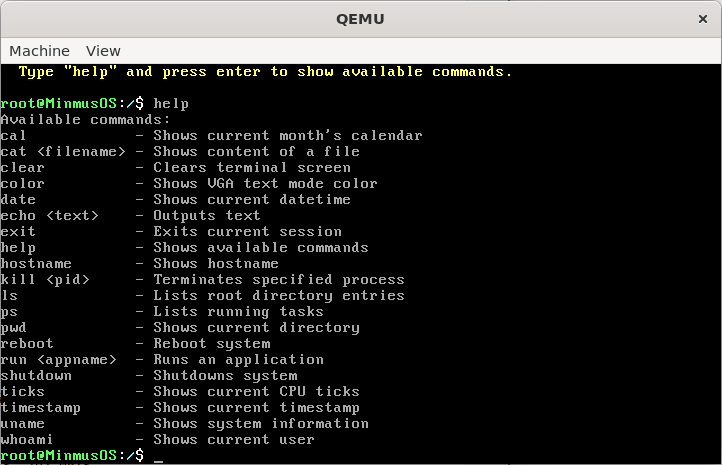
\includegraphics[width=0.8\textwidth]{figures/HelpCommandPresentation.png}
    \caption{Help命令演示}
    \label{fig:HelpCommandPresentation}
\end{figure}

\subsubsection{Shell 数据结构}

Shell 结构(\cref{lst:ShellDataStructure})定义了操作系统的命令行界面,包含三个成员:buffer(一个256字符的数组,用于存储用户输入的命令行文本)、arg(一个11字符的数组,专门用于解析命令参数)、和 cursor(一个 usize 类型,记录当前用户输入的位置)。这个结构体提供了基础的文本输入存储和命令解析功能,使得操作系统能够接收、处理和响应用户的命令操作。

Shell 的实现需要定义三个常量(\cref{lst:ShellConstantDefinitions}),用于操作系统中应用程序的加载和执行管理。它们的作用如下:

\begin{listing}[htbp]
    \begin{minted}{rust}
const APP_TARGET: u32 = 0x00A00000;
const APP_SIZE: u32 = 0x00010000;
const APP_SIGNATURE: u32 = 0xB16B00B5;
    \end{minted}
    \caption{Shell常量定义}\label{lst:ShellConstantDefinitions}
\end{listing}

\begin{enumerate}
    \item \texttt{APP\_TARGET}:表示应用程序在内存中的目标加载地址。操作系统在加载应用程序时,会将其放置在这个内存地址开始的位置。
    \item \texttt{APP\_SIZE}:表示每个应用程序的大小上限(64KB)。这个大小用于划分内存区域,以确保每个应用程序在独立的内存空间中运行,避免相互干扰。
    \item \texttt{APP\_SIGNATURE}:这是一个标识符,用于验证加载的文件是否为有效的可执行文件。操作系统在加载应用程序后,会检查这个签名,以确认该文件确实是一个可以执行的应用程序。
\end{enumerate}

SHELL 是一个可变的静态变量(\cref{lst:ShellStaticVariable}),用于全局管理操作系统的命令行界面(Shell)的状态。SHELL 使用了 mut 关键字,表示该静态变量是可变的。这意味着操作系统可以在运行时动态地更新 SHELL 的状态,例如响应用户输入或执行命令时。SHELL 作为一个全局的 Shell 实例,使得操作系统中的各个模块可以通过访问这个变量来控制和管理命令行界面。它在整个系统中保持单一实例,以便统一管理 Shell 的行为和状态。

\begin{listing}[htbp]
    \begin{minted}{rust}
pub static mut SHELL: Shell = Shell {
    buffer: [0 as char; 256],
    arg: [0 as char; 11],
    cursor: 0,
};
    \end{minted}
    \caption{SHELL静态变量}\label{lst:ShellStaticVariable}
\end{listing}

Shell 实现了如下方法:

\begin{enumerate}
    \item \textbf{init方法}:init 方法用于初始化 Shell 的状态。它将 buffer 清空为全零,并将 cursor 重置为 0,然后通过 PRINTER 设置命令提示符的颜色和格式。具体来说,它设置提示符为 “root@MinmusOS:/\$”,使用不同的颜色(如绿色、白色、青色等)分别标识用户名、主机名、目录和提示符符号。这个方法确保每次命令输入后,Shell 界面都会重新初始化并显示提示符,等待用户输入新的命令。
    \item \textbf{add方法}:add 方法将用户输入的字符 c 添加到 buffer 的当前位置(由 cursor 指定),然后将 cursor 向前移动一位。它同时使用 \texttt{lib::print!} 输出该字符,显示在屏幕上。这个方法用于逐个收集用户输入的命令字符,并在输入时即时显示。
    \item \textbf{backspace方法}:backspace 方法用于处理用户按下退格键的情况。它会将 cursor 位置向后移动一位,并将该位置的字符从 buffer 中删除(即设置为 0 as char),同时调用 \texttt{PRINTER.delete()} 从屏幕上移除最后一个字符。这个方法确保用户可以删除输入的字符。
    \item \textbf{enter方法}:enter 方法在用户按下回车键时调用。它首先调用 \texttt{PRINTER.new\_line()} 在屏幕上换行,然后调用 \texttt{interpret()} 方法解析和执行当前 buffer 中的命令,最后再次调用 \texttt{init()} 方法重置 Shell 状态并显示新的提示符,准备接收下一条命令。
    \item \textbf{interpret方法}:interpret 方法负责解析并执行 buffer 中的命令。它通过检查 buffer 是否匹配特定的命令来决定执行相应的操作(如 cal,cat,ls,run 等)。如果命令匹配,调用对应的函数执行命令逻辑;如果命令未匹配,显示“命令未找到”的错误信息。这个方法是 Shell 的核心,处理和响应用户输入的命令。
    \item \textbf{cat方法}:cat 方法用于显示文件内容。它从 buffer 中提取文件名参数,并调用 FAT 文件系统驱动搜索文件。如果文件存在,读取文件内容并显示在屏幕上;如果文件不存在,显示“文件未找到”的错误信息。这个方法通过操作文件系统,使得用户可以查看文本文件的内容。关于cat命令的实现详见\cref{sec:CatCommand}。
    \item \textbf{run方法}:run 方法用于运行指定的应用程序。它从 buffer 中提取应用程序名称,并调用 FAT 文件系统驱动查找应用程序文件。如果文件存在且签名正确,将其加载到内存的特定位置,并将其作为任务添加到任务管理器中执行。如果文件签名不正确,显示“该文件不是有效的可执行文件”的错误信息;如果文件不存在,显示“应用程序未找到”的错误信息。这个方法实现了操作系统中应用程序的加载与执行。关于run命令的实现详见\cref{sec:RunCommand}。
    \item \textbf{is\_command方法}:is\_command 方法用于判断 buffer 中的内容是否与指定的命令字符串匹配(大小写不敏感)。它逐字符比较 buffer 和 command,如果匹配且 buffer 中命令后的字符是空格或终止符,则返回 true;否则返回 false。这个方法用于在 interpret 方法中识别用户输入的命令,并决定执行相应的操作。
\end{enumerate}

\begin{listing}[htbp]
    \begin{minted}{rust}
pub struct Shell {
    buffer: [char; 256],
    arg: [char; 11],
    cursor: usize,
}

impl Shell {
    pub fn init(&mut self) { ... }

    pub fn add(&mut self, c: char) {
        self.buffer[self.cursor] = c;
        self.cursor += 1;
        lib::print!("{}", c);
    }

    pub fn backspace(&mut self) {
        if self.cursor > 0 {
            unsafe {
                PRINTER.delete();
            }
            self.cursor -= 1;
            self.buffer[self.cursor] = 0 as char;
        }
    }

    pub fn enter(&mut self) {
        unsafe {
            PRINTER.new_line();
        }
        self.interpret();
        self.init();
    }

    #[allow(unused_unsafe)]
    fn interpret(&mut self) { ... }

    unsafe fn cat(&mut self, b: &[char]) { ... }

    unsafe fn run(&mut self, b: &[char]) { ... }

    fn is_command(&self, command: &str) -> bool {
        let command_len: usize = command.len();
        for (i, command_char) in command.chars().enumerate() {
            let buffer_char: char = self.buffer[i].to_ascii_lowercase();
            if buffer_char == '\0' || buffer_char != command_char.to_ascii_lowercase() {
                return false;
            }
        }
        self.buffer[command_len].to_ascii_lowercase() == ' ' || self.buffer[command_len] == '\0'
    }
}
    \end{minted}
    \caption{\texttt{Shell}数据结构}\label{lst:ShellDataStructure}
\end{listing}

\subsubsection{cal 命令}

kernel/src/shell/cal.rs 实现了 cal 命令。cal 命令的实现分为以下几个步骤:

\begin{enumerate}
    \item \textbf{获取当前日期信息}:在 calendar 函数的开头,通过调用 Time::init() 获取当前时间的实例,然后分别提取当前的年、月和日。这个时间信息是接下来生成日历的基础。
    \item \textbf{确定月份标题}:使用 match 表达式根据 month 值确定月份的名称,如“January”、“February”等。然后将月份名称与年份一起打印在日历的顶部,作为日历的标题。
    \item \textbf{计算月份的第一天}:使用 Zeller's Congruence 算法(\cref{lst:ZellerCongruenceAlgorithm})计算出当月第一天是星期几。这一步得到一个从 0 到 6 的数值,表示星期一到星期日。这是日历对齐的关键,用于决定该月的日期从星期几开始显示。
    \item \textbf{确定当月的天数}:通过 match 表达式,根据月份值确定当月的天数。如果是二月,还需判断该年是否为闰年,从而决定二月是 28 天还是 29 天。
    \item \textbf{生成和显示日历}:首先,根据计算出的 first\_day\_of\_month 在日历的第一行前打印适当数量的空格,然后逐日打印该月的日期。打印过程中,如果当前日期正好是当天,则会高亮显示(将日期文字设为黄色)。每当日期跨过一个星期时,换行继续打印,直到打印完当月所有日期。
    \item \textbf{最终输出}:日历打印完成后,通过调用 \texttt{lib::println!() }确保日历输出的最后一行与后续输出之间有一个空行隔开。
\end{enumerate}

\begin{listing}[htbp]
    \begin{minted}{rust}
let first_day_of_month: usize = {
    let (y, m): (i32, u8) = if month < 3 { (year as i32 - 1, month + 12) } else { (year as i32, month) };
    let k: i32 = y % 100;
    let j: i32 = y / 100;
    let h: i32 = (1 + (13 * (m as i32 + 1)) / 5 + k + k / 4 + j / 4 + 5 * j) % 7;
    ((h + 5) % 7) as usize
};
    \end{minted}
    \caption{Zeller's Congruence 算法}\label{lst:ZellerCongruenceAlgorithm}
\end{listing}

\subsubsection{cat <filename> 命令}\label{sec:CatCommand}

\cref{lst:CatMethod}实现了cat命令:

\begin{enumerate}
    \item \textbf{解析命令参数}:当用户输入 cat <filename> 时,buffer 中会包含命令和文件名。cat 函数首先需要从 buffer 中提取文件名。它通过定位文件名的起始和结束位置,确保能够正确解析用户输入的文件名。如果文件名解析失败(例如没有提供文件名或文件名格式不正确),函数会显示用法提示“Usage: cat <filename>”并返回。
    \item \textbf{设置文件名参数}:将提取的文件名字符逐个复制到 Shell 结构体的 arg 数组中,确保文件名被正确存储。超过 arg 数组长度的部分会被截断,同时在未使用的部分填充0以确保字符串正确结束。
    \item \textbf{查找文件}:cat 函数通过 \texttt{FAT.acquire()} 获取当前使用的 FAT 文件系统驱动,然后调用 texttt{fat.search\_file(\&self.arg)} 在文件系统中查找与 arg 中指定的文件名匹配的文件条目 Entry。如果没有找到对应的文件,会显示错误信息“File not found!”,并结束命令执行。
    \item \textbf{读取和显示文件内容}:如果找到文件,cat 函数会将文件内容读取到缓冲区并打印在屏幕上。通过调用 \texttt{fat.read\_file\_to\_buffer(entry)},文件内容会被读取到文件系统的缓冲区 \texttt{fat.buffer} 中,然后逐个字符地打印出来,直到文件结束。
    \item \textbf{释放文件系统驱动}:在操作结束后,cat 函数调用 \texttt{FAT.free()} 释放文件系统驱动,使其可以被其他操作使用,从而确保系统资源的合理管理。
    \item \textbf{结束处理}:最后,cat 函数调用 \texttt{lib::println!()} 输出一个空行,以保持命令行界面的整洁,标志命令执行的结束。
\end{enumerate}

\begin{listing}[htbp]
    \begin{minted}{rust}
unsafe fn cat(&mut self, b: &[char]) {
    ...
    let fat: &FatDriver = FAT.acquire();
    let entry: &Entry = fat.search_file(&self.arg);
    if entry.name[0] != 0 {
        fat.read_file_to_buffer(entry);
        for c in fat.buffer {
            if c != 0 {
                lib::print!("{}", c as char);
            }
        }
        lib::println!();
    } else {
        PRINTER.set_colors(COLOR_LIGHT_RED, COLOR_BLACK);
        lib::println!("File not found!");
        PRINTER.reset_colors();
    }
    FAT.free();
}
    \end{minted}
    \caption{cat方法}\label{lst:CatMethod}
\end{listing}

\subsubsection{clear 命令}

clear 命令的实现非常简单,当用户输入 clear 命令时,程序通过 \texttt{is\_command("clear")} 检查用户输入的命令是否为 clear。如果匹配,程序调用 \texttt{PRINTER.clear()} 方法,该方法负责清空终端屏幕内容,从而实现屏幕的清除效果。整个过程通过直接调用打印系统的清除功能,确保命令行界面恢复到一个干净的状态。

\subsubsection{color 命令}

color 命令的实现通过遍历前景色(fg)和背景色(bg)的所有可能组合(共16种),并使用 \texttt{PRINTER.set\_colors(fg, bg)} 设置不同的颜色组合。每种组合都在屏幕上显示其对应的颜色代码(例如“01”表示前景色为1,背景色为0),以可视化方式展示所有可能的颜色配置。最后,调用 \texttt{PRINTER.reset\_colors()} 恢复默认颜色设置。这个命令主要用于展示终端支持的颜色选项和效果。

\subsubsection{date 命令}

date 命令的实现通过调用 \texttt{Time::init()} 获取当前系统时间,并提取年、月、日、小时、分钟和秒等时间信息。然后使用 \texttt{lib::println!} 以 YYYY-MM-DD HH:MM:SS UTC 的格式将时间打印到终端上,显示当前的系统日期和时间。整个过程通过简单的时间提取和格式化输出,实现了显示当前日期和时间的功能。

\subsubsection{echo <text> 命令}

echo 命令的实现(\cref{lst:EchoMethod})用于在终端中输出用户输入的文本。函数首先跳过命令本身(echo 及其后的空格),然后逐字符遍历用户输入的文本字符。如果遇到空格字符且前一个字符也是空格,则跳过该空格;否则,将字符输出到终端。这样做的目的是避免输出连续的多个空格。在所有字符处理完成后,调用 \texttt{lib::println!()} 输出换行符,确保命令执行后的光标位置正确。通过这种方式,echo 命令可以将用户输入的文本整齐地显示在终端上。

\begin{listing}[htbp]
    \begin{minted}{rust}
pub fn echo(b: &[char]) {
    let mut last_was_space = true;
    for &ch in b.iter().skip(5) {
        if ch == '\0' {
            break;
        }
        if ch == ' ' {
            if !last_was_space {
                lib::print!(" ");
                last_was_space = true;
            }
        } else {
            lib::print!("{}", ch);
            last_was_space = false;
        }
    }
    lib::println!();
}
    \end{minted}
    \caption{echo方法}\label{lst:EchoMethod}
\end{listing}

\subsubsection{exit 命令}

exit 命令用于退出当前会话。实现时,通过使用内联汇编指令 \texttt{core::arch::asm!},将特定值输出到 I/O 端口,以触发系统退出或关机。这是直接通过硬件端口操作实现退出功能。

\subsubsection{help 命令}

help 命令用于显示系统中可用的所有命令及其简要描述。实现时,直接通过 \texttt{lib::println!} 输出预先定义好的帮助文本 HELP,让用户查看命令列表和使用说明。

\subsubsection{hostname 命令}

hostname 命令用于显示当前操作系统的主机名。实现时,通过 \texttt{lib::println!("MinmusOS")} 输出主机名为“MinmusOS”,让用户了解当前系统的标识。

\subsubsection{kill <pid> 命令}

\cref{lst:KillMethod}实现了kill命令:

\begin{enumerate}
    \item \textbf{解析命令参数}:当用户输入 kill <pid> 命令时,首先需要从输入的命令行中提取 PID 参数。函数从 b 中跳过命令本身(即 kill 及其后面的空格字符)来定位 PID 的起始位置 start。如果 PID 的起始位置不合法(即没有提供有效的 PID),函数会立即返回,并显示“Usage: kill <pid>”提示用户正确的使用方法。
    \item \textbf{验证和解析 PID}:一旦 PID 的起始位置确定,函数继续向后寻找 PID 的结束位置。通过再次遍历 b,寻找第一个空格或空字符来确定 PID 的结束位置 end。在提取出 PID 的字符序列后,函数将逐字符检查并将其转换为整数 task\_id。在这个过程中,如果发现任何非数字字符,函数会判定 PID 输入无效,并立即返回,同时显示“Please enter a valid PID (1-31)”的错误信息。
    \item \textbf{验证 PID 范围}:在成功解析并转换 PID 为整数后,函数会进一步检查该 PID 是否在合法范围内,即是否在 1 到 MAX\_TASKS 之间。如果 PID 超出了这个范围,函数会显示错误提示“Please enter a valid PID (1-31)”,并结束操作。这一检查确保了用户输入的 PID 是系统内一个有效的任务标识符。
    \item \textbf{移除任务}:kill 命令会调用 \texttt{TASK\_MANAGER.remove\_task(task\_id)} 来终止系统中对应的任务,如果 PID 验证通过且在合法范围内。TASK\_MANAGER 是一个全局的任务管理器,负责管理所有运行中的任务。通过调用 remove\_task 方法,系统会根据用户提供的 PID 查找到对应的任务,并将其从任务队列中移除。移除成功后,函数会使用 \texttt{lib::println!("Task (PID \{\}) has been removed.", task\_id)} 输出确认信息,告知用户任务已成功终止。
    \item \textbf{输出与提示}:在整个命令执行过程中,kill 函数使用 PRINTER 进行文本输出。PRINTER 负责控制终端的显示,包括设置文本颜色和输出内容。为了区分正常操作和错误信息,kill 命令在输出错误信息时,会将文本颜色设置为 COLOR\_LIGHT\_RED,而在输出提示信息时,会将颜色设置为 COLOR\_LIGHT\_MAGENTA。在所有操作完成后,函数会调用 \texttt{PRINTER.reset\_colors()} 将颜色恢复到默认状态。通过这种方式,kill 命令确保了用户在使用过程中可以清晰地接收到正确的反馈信息,增强了用户体验的友好性和操作的安全性。
\end{enumerate}

\begin{listing}[htbp]
    \begin{minted}{rust}
pub fn kill(b: &[char]) {
    ...
    for i in start + 5..end {
        if b[i].is_digit(10) { task_id = task_id * 10 + (b[i] as u8 - b'0') as usize; }
        else { is_valid_id = false; break; }
    }
    if is_valid_id {
        if task_id > 0 && task_id < MAX_TASKS as usize {
            unsafe {
                if !TASK_MANAGER.tasks[task_id].running {
                    PRINTER.set_colors(COLOR_LIGHT_RED, COLOR_BLACK);
                    lib::println!("Task with PID {} not found!", task_id);
                    PRINTER.reset_colors();
                    return;
                }
                TASK_MANAGER.remove_task(task_id);
                lib::println!("Task (PID {}) has been removed.", task_id);
            }
        } else {
            unsafe { PRINTER.set_colors(COLOR_LIGHT_RED, COLOR_BLACK); }
            lib::println!("Please enter a valid PID (1-31).");
            unsafe { PRINTER.reset_colors(); }
        }
    } else {
        unsafe { PRINTER.set_colors(COLOR_LIGHT_RED, COLOR_BLACK); }
        lib::println!("Please enter a valid PID (1-31).");
        unsafe { PRINTER.reset_colors(); }
    }
}
    \end{minted}
    \caption{kill方法}\label{lst:KillMethod}
\end{listing}

\subsubsection{ls 命令}

ls 命令用于列出根目录中的所有文件和目录项。实现时,通过调用 \texttt{FAT.acquire()} 获取文件系统驱动,并使用 \texttt{list\_entries()} 方法列出根目录中的所有条目。操作完成后,调用 \texttt{FAT.free()} 释放文件系统资源,确保系统资源的有效管理。

\subsubsection{ps 命令}

ps 命令用于显示当前系统中所有正在运行的任务列表。实现时,调用全局任务管理器 TASK\_MANAGER 的 \texttt{list\_tasks()} 方法,该方法会遍历系统中的所有任务并将其状态输出到终端,帮助用户查看系统中正在执行的任务。

\subsubsection{pwd 命令}

pwd 命令用于显示当前工作目录。在这个实现中,命令直接输出根目录“/”,表明当前工作目录为系统的根目录。由于此 Shell 环境中没有复杂的目录结构,pwd 命令只返回根目录。

\subsubsection{reboot 命令}

reboot 命令用于重新启动系统。实现时,通过内联汇编 \texttt{core::arch::asm!} 发送特定命令到系统的 I/O 端口,触发硬件重启。这个直接的硬件操作确保了系统能够立即重新启动。

\subsubsection{run <appname> 命令}\label{sec:RunCommand}

\cref{lst:RunMethod}实现了run命令:

\begin{enumerate}
    \item \textbf{解析应用程序名称}:run 方法首先从用户输入的命令行中提取应用程序的名称。通过跳过 run 及其后的空格字符,定位应用程序名称的起始位置 start。如果没有提供有效的应用程序名称,或者名称格式不正确,方法会立即返回并显示用法提示“Usage: run <appname>”。
    \item \textbf{设置应用程序名称参数}:在成功提取到应用程序名称后,方法将其逐字符复制到 Shell 结构体的 arg 数组中,并确保名称字符串以 0 结束。如果应用程序名称超出 arg 数组的长度,则会被截断。
    \item \textbf{查找应用程序文件}:run 方法接下来会在文件系统中查找指定名称的应用程序文件。首先通过 \texttt{FAT.acquire()} 获取 FAT 文件系统驱动,然后调用 \texttt{fat.search\_file(\&self.arg)} 在文件系统中搜索与 arg 数组中存储的名称匹配的文件条目。如果找不到对应的文件,方法会显示“Application not found!”的错误信息,并结束操作。
    \item \textbf{加载并执行应用程序}:如果找到应用程序文件,方法会尝试将其加载到内存中并执行。首先,方法通过 \texttt{TASK\_MANAGER.get\_free\_slot()} 获取一个空闲的任务槽位,并计算应用程序的加载目标地址 target。然后,设置分页表 TABLES[8] 并调用 \texttt{PAGING.set\_table},将应用程序加载到指定的内存位置。如果应用程序文件包含有效的签名(与 APP\_SIGNATURE 匹配),run 方法会通过 \texttt{TASK\_MANAGER.add\_task(target + 4)} 将其作为一个新任务添加到任务管理器中执行。如果签名不匹配,方法会显示“This file is not a valid executable!”的错误信息。
    \item \textbf{清理与释放资源}:最后,无论运行应用程序是否成功,方法都会调用 \texttt{FAT.free()} 释放文件系统驱动,以确保资源的合理使用和系统的稳定性。
\end{enumerate}

\begin{listing}[htbp]
    \begin{minted}{rust}
unsafe fn run(&mut self, b: &[char]) {
    let start: usize = b.iter().skip(4).position(|&c| c != ' ' && c != '\0').unwrap_or(b.len());
    if start + 4 >= b.len() {
        unsafe {
            PRINTER.set_colors(COLOR_LIGHT_MAGENTA, COLOR_BLACK);
        }
        lib::println!("Usage: run <appname>");
        unsafe {
            PRINTER.reset_colors();
        }
        return;
    }
    let end: usize = b.iter().skip(start + 4).position(|&c| c == ' ' || c == '\0').map_or(b.len(), |p| p + start + 4);
    if end <= start + 4 {
        unsafe {
            PRINTER.set_colors(COLOR_LIGHT_MAGENTA, COLOR_BLACK);
        }
        lib::println!("Usage: run <appname>");
        unsafe {
            PRINTER.reset_colors();
        }
        return;
    }
    let mut j: usize = 0;
    for i in start + 4..end {
        self.arg[j] = b[i];
        j += 1;
    }
    for i in j..self.arg.len() {
        self.arg[i] = '\0';
    }
    let fat: &FatDriver = FAT.acquire();
    let entry: &Entry = fat.search_file(&self.arg);
    if entry.name[0] != 0 {
        let target: u32 = APP_TARGET + (TASK_MANAGER.get_free_slot() as u32 * APP_SIZE);
        TABLES[8].set(target);
        PAGING.set_table(8, &TABLES[8]);
        fat.read_file_to_target(&entry, target as *mut u32);
        if *(target as *mut u32) == APP_SIGNATURE {
            TASK_MANAGER.add_task(target + 4);
        } else {
            unsafe { PRINTER.set_colors(COLOR_LIGHT_RED, COLOR_BLACK); }
            lib::println!("This file is not a valid executable!");
            unsafe { PRINTER.reset_colors(); }
        }
    } else {
        PRINTER.set_colors(COLOR_LIGHT_RED, COLOR_BLACK);
        lib::println!("Application not found!");
        PRINTER.reset_colors();
    }
    FAT.free();
}
    \end{minted}
    \caption{run方法}\label{lst:RunMethod}
\end{listing}

\subsubsection{shutdown 命令}

shutdown 命令用于关闭系统。实现时,通过内联汇编 \texttt{core::arch::asm!},将特定的值输出到 I/O 端口,触发系统的关机操作。这是一个直接的硬件控制命令,用于立即停止系统的运行。

\subsubsection{ticks 命令}

ticks 命令用于显示自系统启动以来的CPU时钟滴答数。实现时,通过调用 \texttt{Time::init()} 初始化时间模块,然后使用 \texttt{get\_ticks()} 方法获取当前的滴答数,并通过 \texttt{lib::println!} 将其输出到终端,供用户查看。

\subsubsection{timestamp 命令}

timestamp 命令用于显示当前的时间戳。实现时,同样调用 \texttt{Time::init()} 初始化时间模块,并使用 \texttt{get\_timestamp()} 方法获取当前的 Unix 时间戳,表示自1970年1月1日以来的秒数。然后将其通过 \texttt{lib::println!} 输出,方便用户查看当前时间戳。

\subsubsection{uname 命令}

uname 命令用于显示操作系统的名称和版本信息。实现时,直接通过 \texttt{lib::println!} 输出操作系统的名称和版本信息,例如“MinmusOS v1.0 IA-32 x86”,以告知用户当前运行的操作系统的基本信息。

\subsubsection{whoami 命令}

whoami 命令用于显示当前用户的身份。实现时,通过 \texttt{lib::println!("root")} 直接输出用户名称“root”,表明当前操作系统的用户身份为超级用户。

\subsection{主启动程序(Main Boot Program)}

\subsection{链接器脚本(Linker Script)}